% Copyright 2004 by Till Tantau <tantau@users.sourceforge.net>.
%
% In principle, this file can be redistributed and/or modified under
% the terms of the GNU Public License, version 2.
%
% However, this file is supposed to be a template to be modified
% for your own needs. For this reason, if you use this file as a
% template and not specifically distribute it as part of a another
% package/program, I grant the extra permission to freely copy and
% modify this file as you see fit and even to delete this copyright
% notice. 

\documentclass{beamer}
% There are many different themes available for Beamer. A comprehensive
% list with examples is given here:
% http://deic.uab.es/~iblanes/beamer_gallery/index_by_theme.html
% You can uncomment the themes below if you would like to use a different
% one:
%\usetheme{AnnArbor}
%\usetheme{Antibes}
%\usetheme{Bergen}
%\usetheme{Berkeley}
%\usetheme{Berlin}
%\usetheme{Boadilla}
%\usetheme{boxes}
%\usetheme{CambridgeUS}
%\usetheme{Copenhagen}
%\usetheme{Darmstadt}
%\usetheme{default}
%\usetheme{Frankfurt}
%\usetheme{Goettingen}
%\usetheme{Hannover}
%\usetheme{Ilmenau}
%\usetheme{JuanLesPins}
%\usetheme{Luebeck}
\usetheme{Madrid}
%\usetheme{Malmoe}
%\usetheme{Marburg}
%\usetheme{Montpellier}
%\usetheme{PaloAlto}
%\usetheme{Pittsburgh}
%\usetheme{Rochester}
%\usetheme{Singapore}
%\usetheme{Szeged}
%\usetheme{Warsaw}

\usepackage{multimedia}
\usepackage{subfig}
%\usebackgroundtemplate{\includegraphics[width= \paperwidth, height=\paperheight]{imagen2}}

\title{Sistema de control autónomo para robot en FPGAs libres}

% A subtitle is optional and this may be deleted
\subtitle{}

\author{Juan Ordóñez Cerezo\inst{1}}
% - Give the names in the same order as the appear in the paper.
% - Use the \inst{?} command only if the authors have different
%   affiliation.

\institute[Universidad de Granada] % (optional, but mostly needed)
{
  \inst{1}%
  Universidad de Granada
}
% - Use the \inst command only if there are several affiliations.
% - Keep it simple, no one is interested in your street address.

\date{}
% - Either use conference name or its abbreviation.
% - Not really informative to the audience, more for people (including
%   yourself) who are reading the slides online

\subject{}
% This is only inserted into the PDF information catalog. Can be left
% out. 

% If you have a file called "university-logo-filename.xxx", where xxx
% is a graphic format that can be processed by latex or pdflatex,
% resp., then you can add a logo as follows:

% \pgfdeclareimage[height=0.5cm]{university-logo}{university-logo-filename}
% \logo{\pgfuseimage{university-logo}}

% Delete this, if you do not want the table of contents to pop up at
% the beginning of each subsection:
\AtBeginSubsection[]
{
  \begin{frame}<beamer>{Outline}
    \tableofcontents[currentsection,currentsubsection]
  \end{frame}
}

% Let's get started
\begin{document}

\begin{frame}
  \begin{center}
  
\includegraphics [width =0.5\textwidth ]{logo_ugr}
  \end{center}
    \begin{center}
	
\includegraphics [width =0.4\textwidth ]{logo_rey}
	\end{center}
  \titlepage
\end{frame}

\begin{frame}{Index}
  \tableofcontents
  % You might wish to add the option [pausesections]
\end{frame}

\section{Contexto}
%%%%%%%%%%%%%%%%%%%%%%%%%%%%%%%%%%%%%%%%%%%%%%%%%%%%%%%%%%%%%%%%%%%%%%%%%%%%%%%

\begin{frame}{Contexto}
	
\end{frame}

\begin{frame}{Planificación y Metodología de trabajo}
	\begin{center}
		\begin{figure}[H]
			\center
			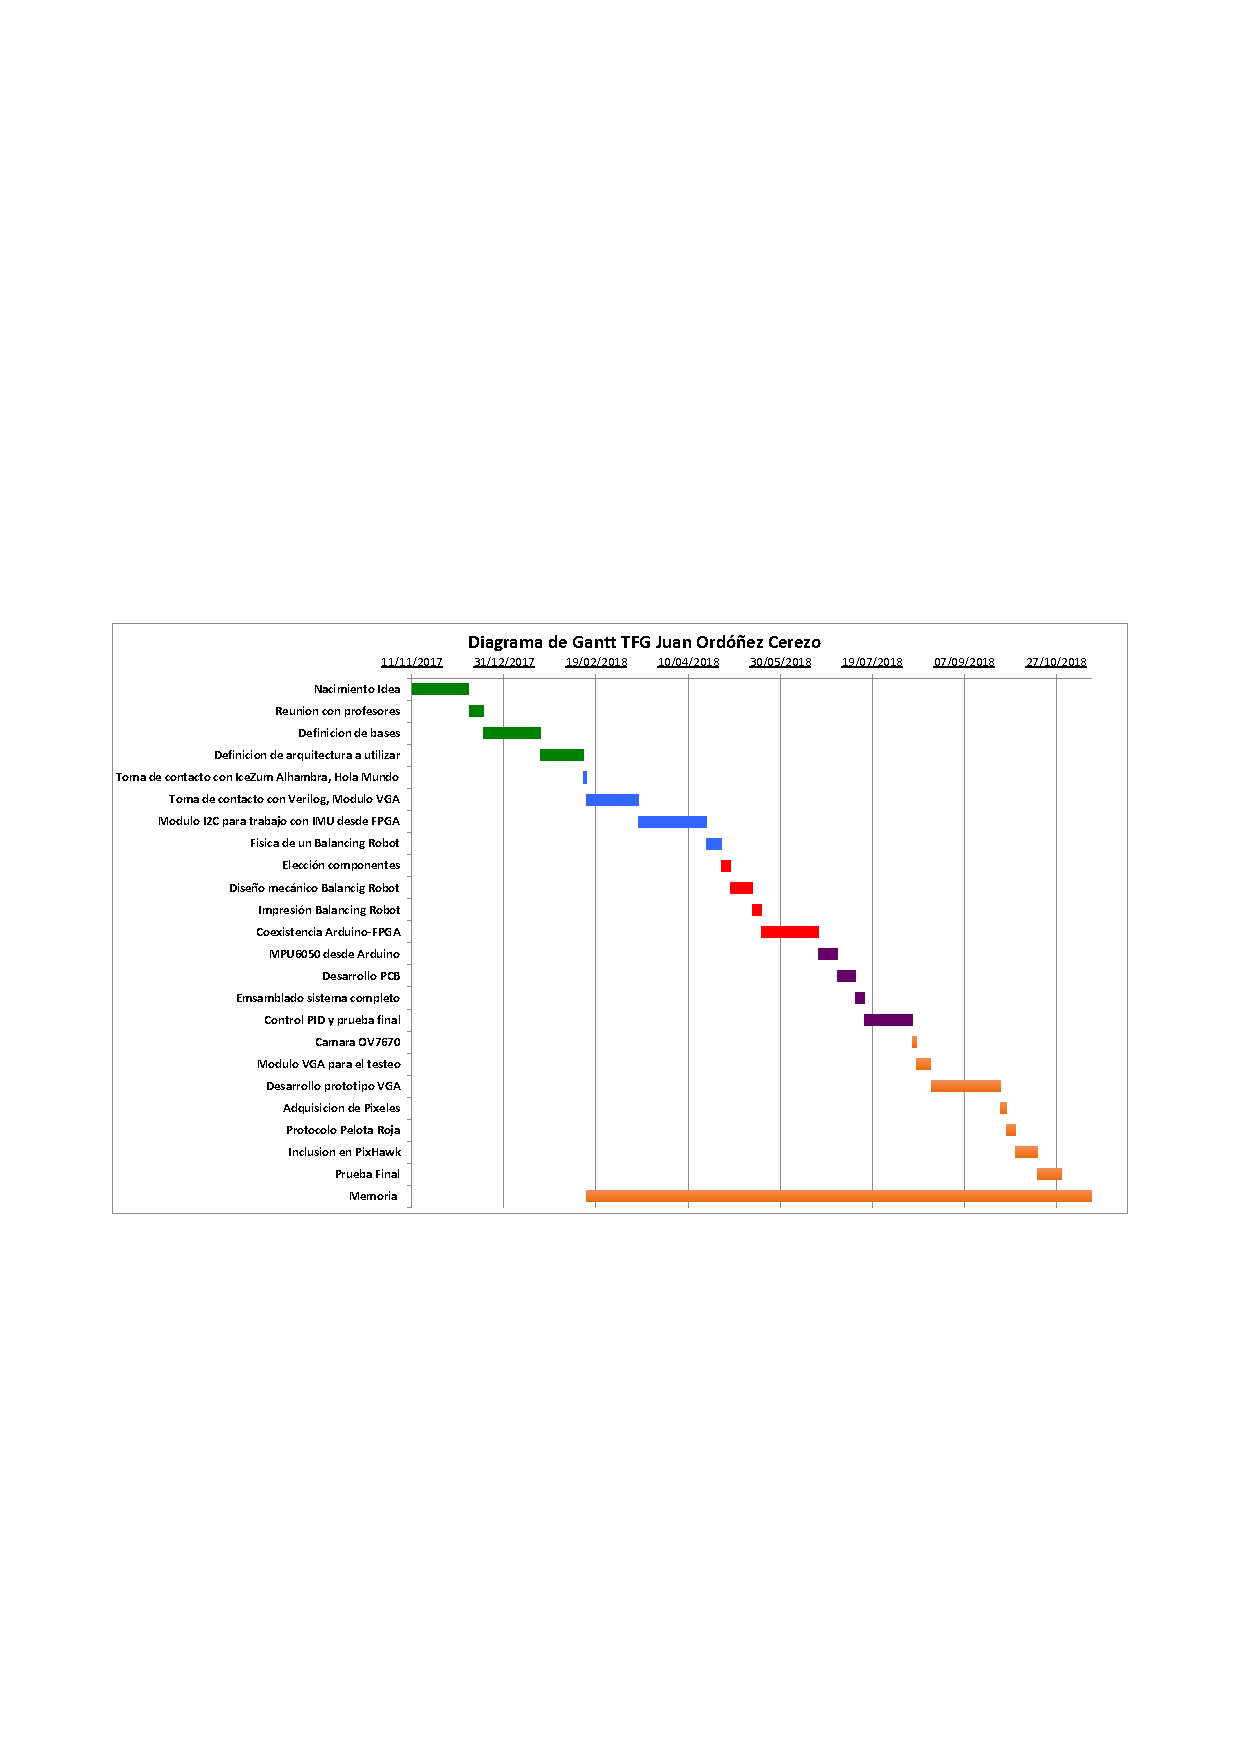
\includegraphics[trim = 1.3cm 0mm 0mm 10.5cm,clip, angle=0, scale = 0.65]{imagenes/Introduction/Gantt.pdf}

		\end{figure}
	\end{center}
\end{frame}

\begin{frame}{Planificación y Metodología de trabajo}
\begin{figure}[H]
	\center	
	\subfloat[GitHub]{
	
\includegraphics[trim = 0mm 0mm 0mm 0mm, clip,scale=0.3]{imagenes/Introduction/github}}
	\subfloat[Appear]{
	
\includegraphics[trim = 0mm 0mm 0mm 0mm, clip,scale=0.2]{imagenes/Introduction/appear}}
\end{figure}
\end{frame}


\begin{frame}{Infraestructura}
	
\end{frame}

\begin{frame}{FPGAs Libres y IceZum Alhambra}
Introducción sobre FPGAs libres y presentación de IceZum con sus carasterísticas breves
\end{frame}
\begin{frame}{IceStudio}
¿Qué es IceStudio y para que nace? Ejemplos de su uso
\end{frame}
\begin{frame}{Objetivos}
Objetivos principales de este trabajo
\end{frame}

%%%%%%%%%%%%%%%%%%%%%%%%%%%%%%%%%%%%%%%%%%%%%%%%%%%%%%%%%%%%%%%%%%%%
\section{Robot Balancín}
\subsection{Diseño del sistema}
\begin{frame}{Diseño del sistema}
\begin{figure}[H]
	\center
	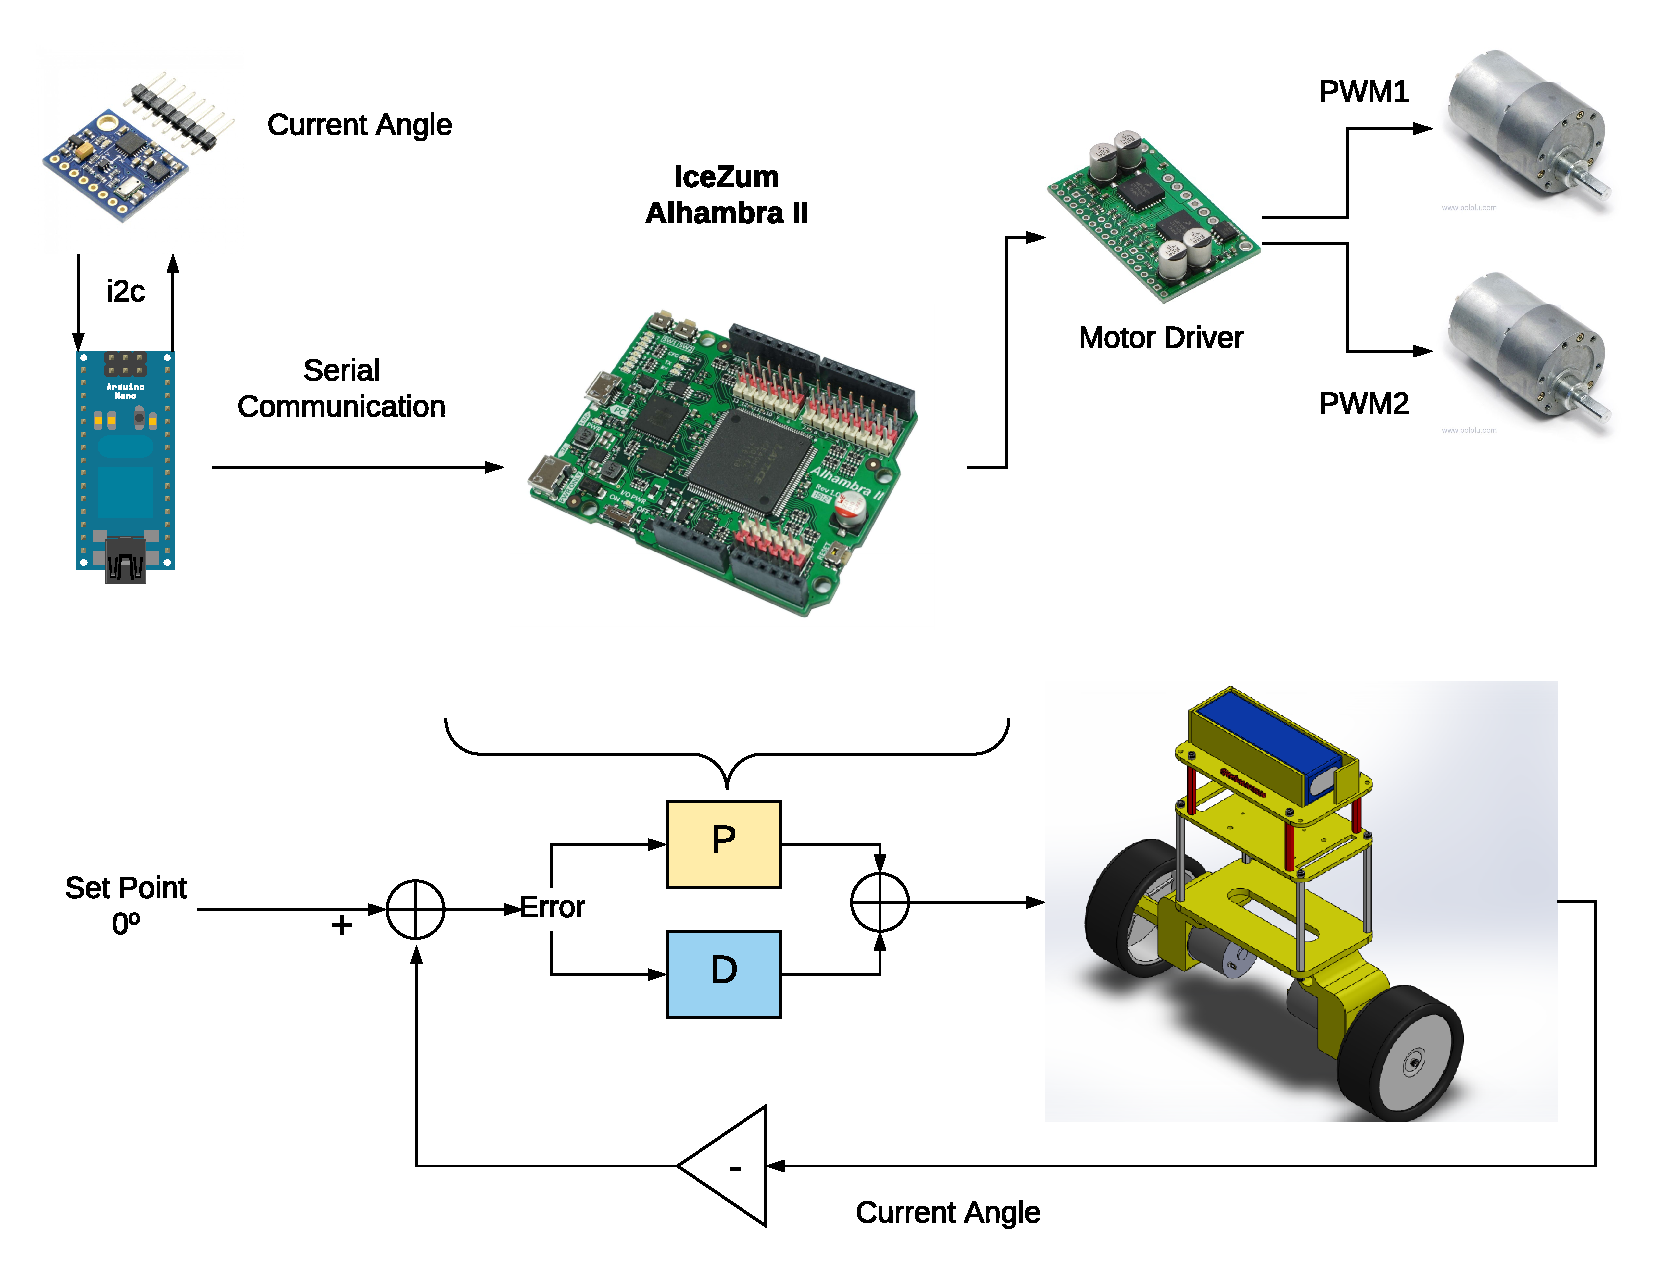
\includegraphics[trim = 0mm 0mm 0mm 0mm, clip,scale=0.3]{imagenes/Balancing_robot/final.pdf}
	\caption{}
	\label{}
\end{figure}
\end{frame}	
\subsection{Implementación del sistema}

\begin{frame}{Estructura mecánica}
\begin{center}
	\begin{figure}[H]
		\center
		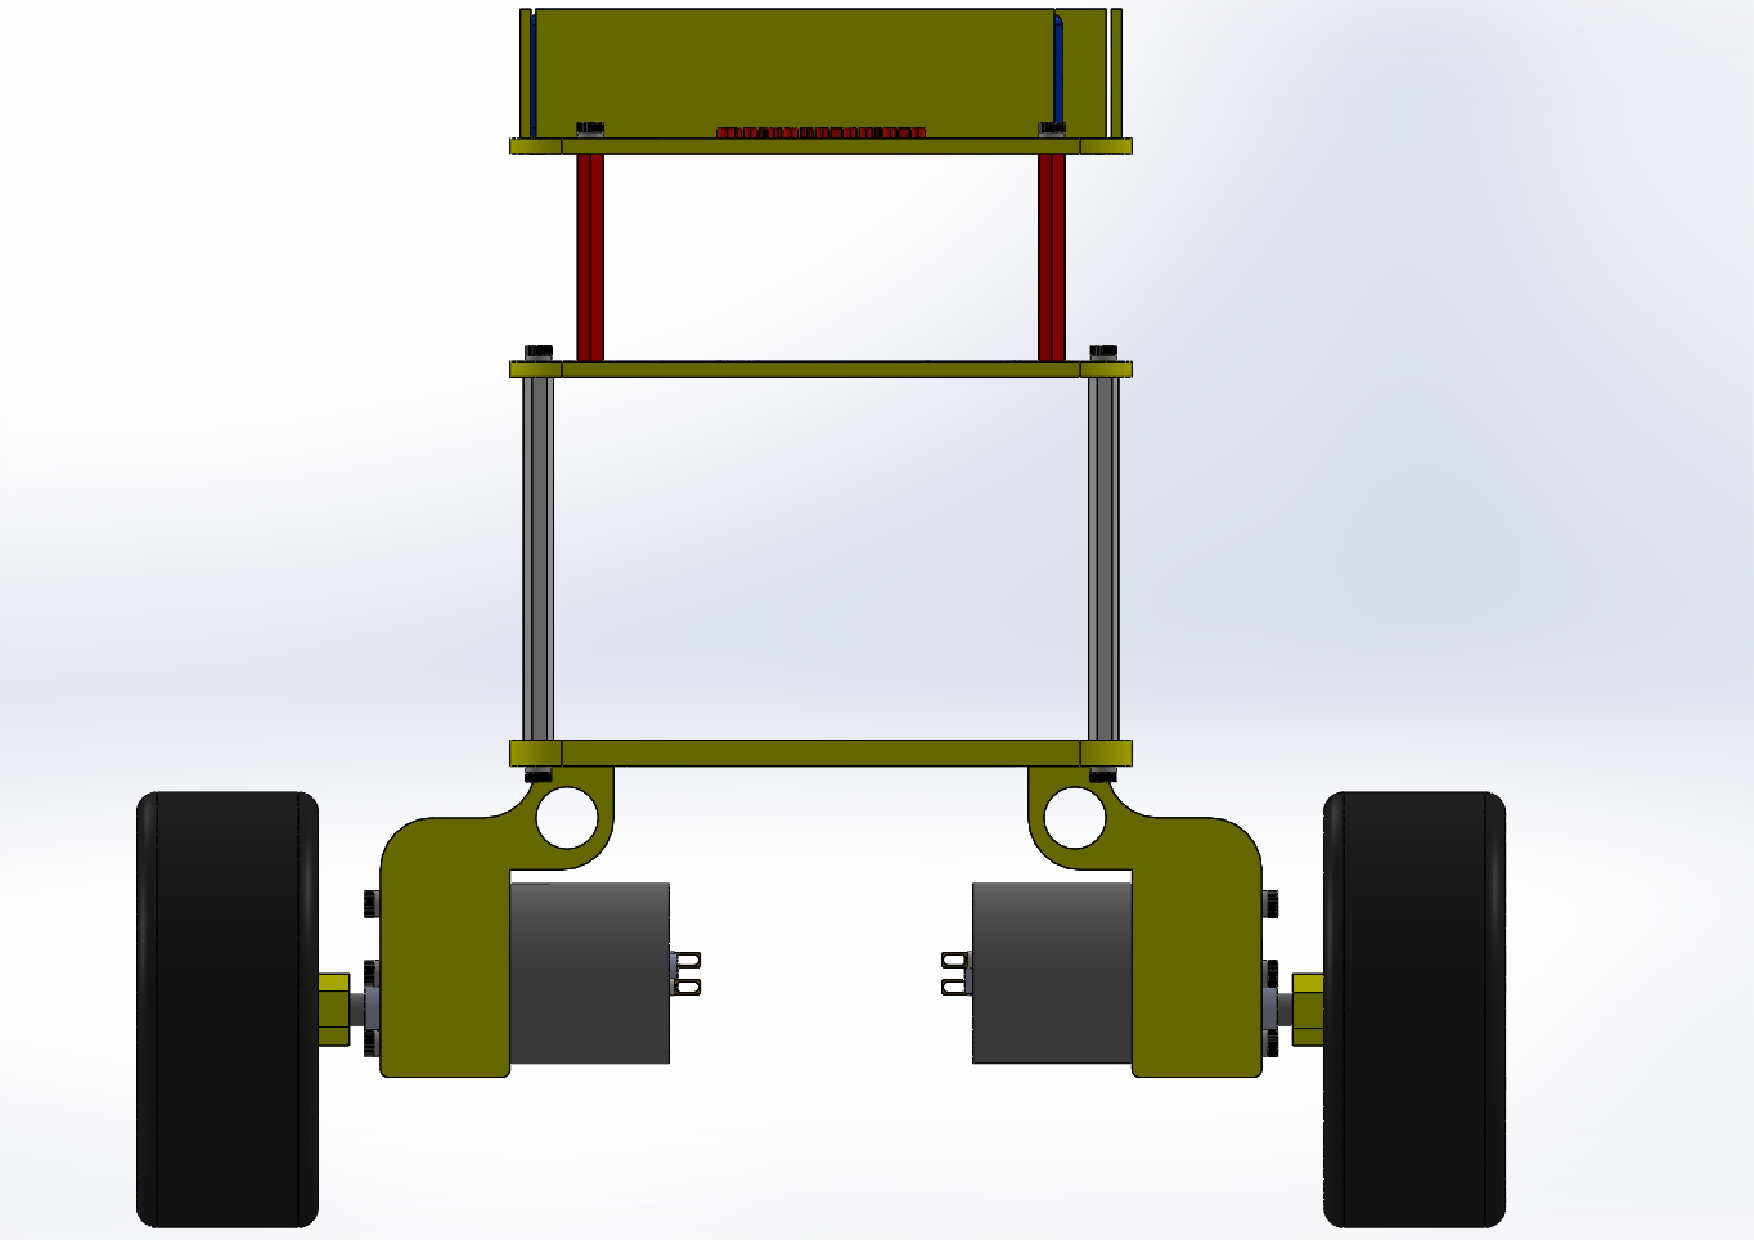
\includegraphics[trim = 1cm 0mm 2.7cm 0mm,clip, angle=0, scale = 0.35]{imagenes/Balancing_Robot/EnsanBalanceFront.PDF}
	\end{figure}
\end{center}
\end{frame}

\begin{frame}{Estructura mecánica}
\begin{center}
	\begin{figure}[H]
		\center
		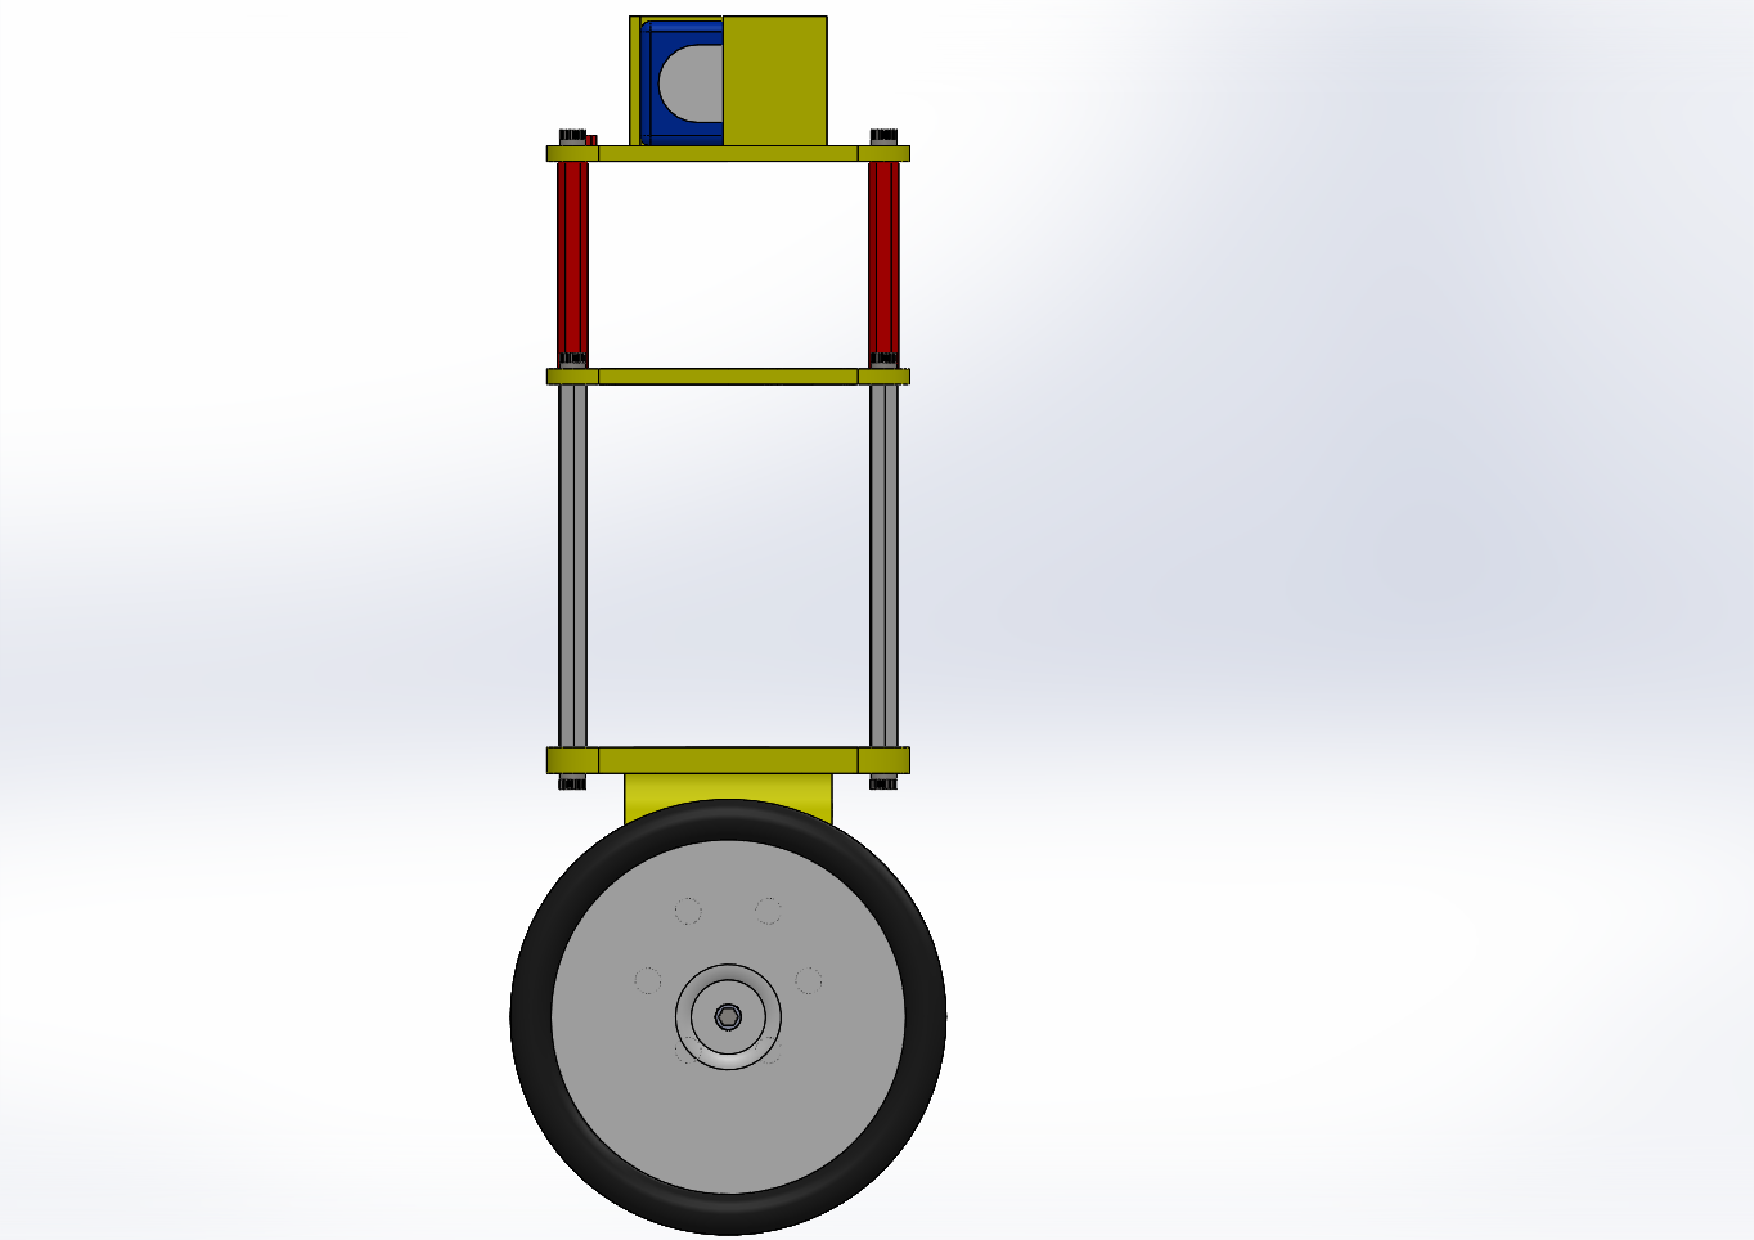
\includegraphics[trim = 5cm 0mm 10cm 0mm,clip, angle=0, scale = 0.35]{imagenes/Balancing_Robot/EnsanBalanceLateral.PDF}
	\end{figure}
\end{center}
\end{frame}

\begin{frame}{Estructura mecánica}
\begin{center}
	\begin{figure}[H]
		\center
		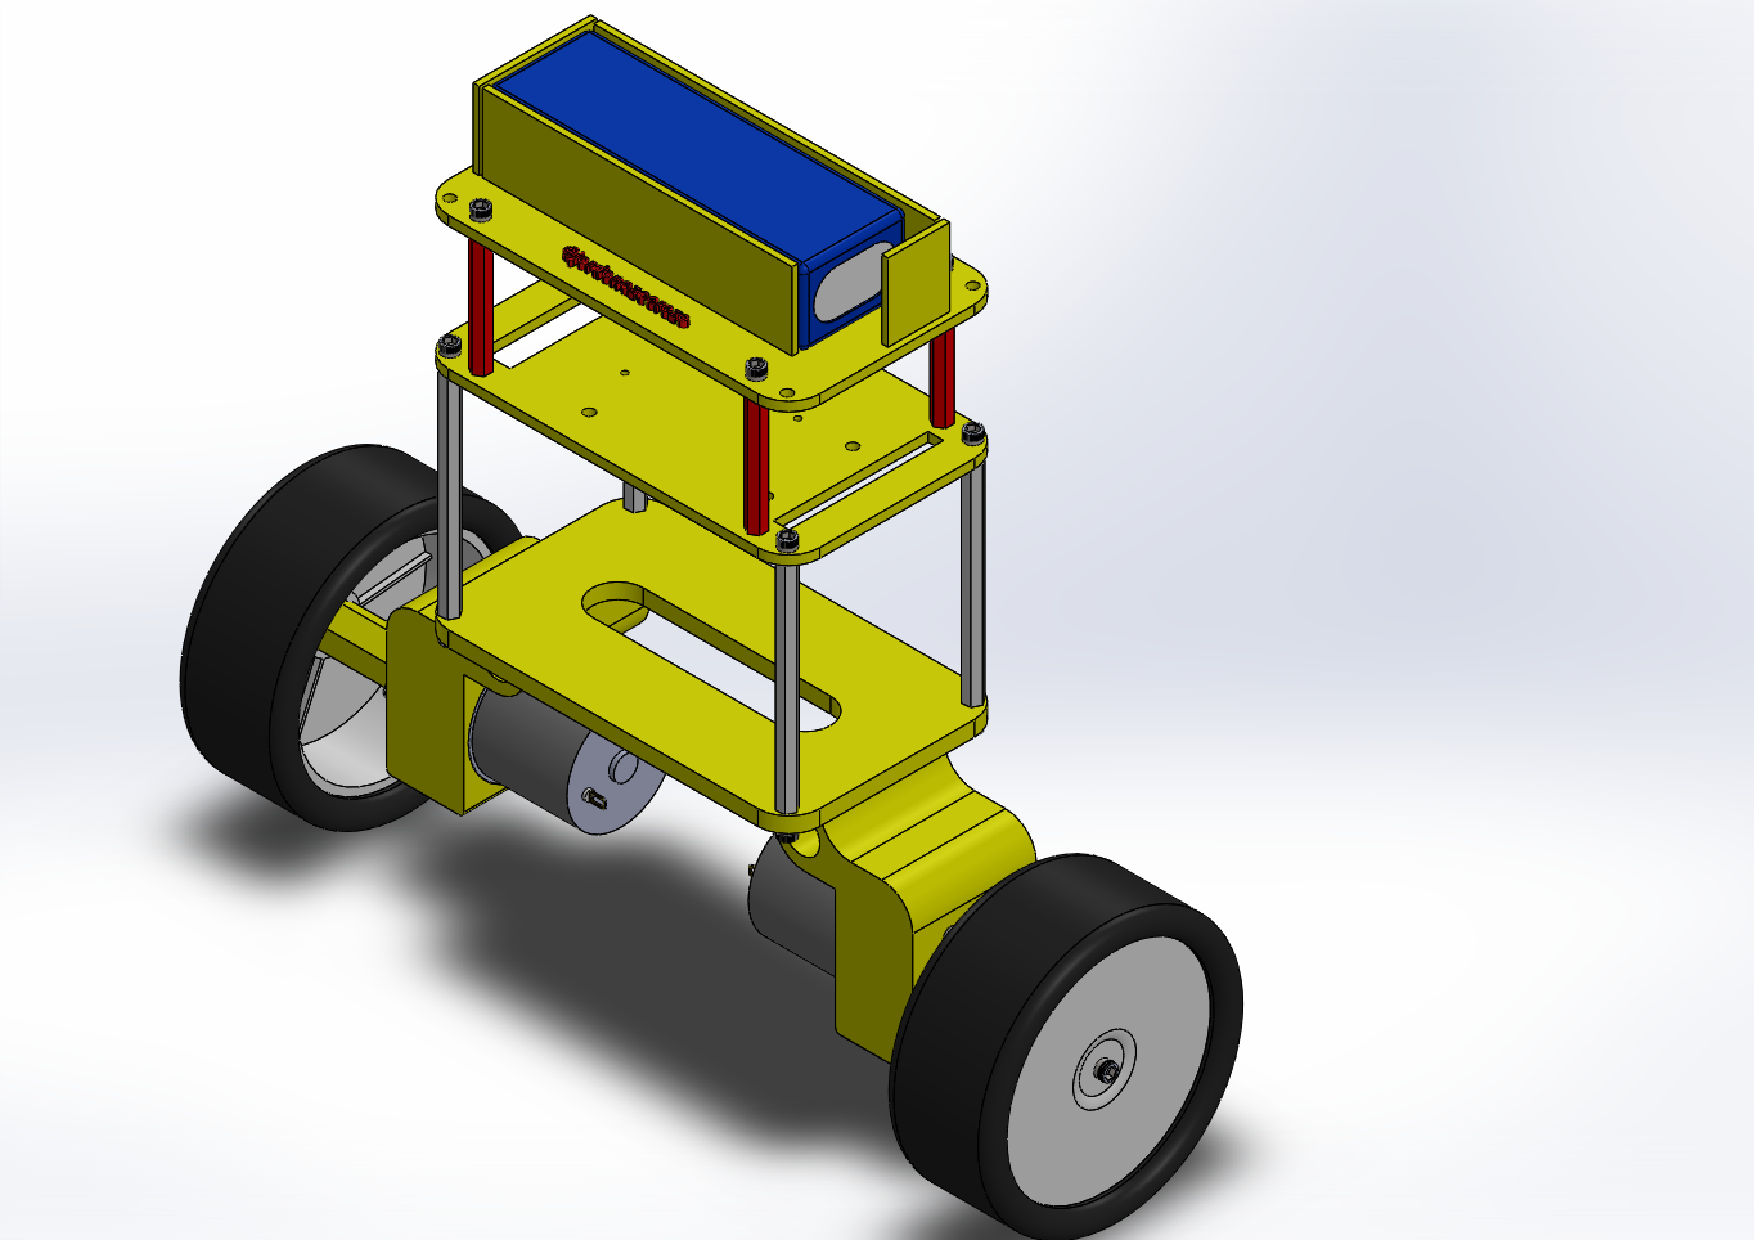
\includegraphics[trim = 2cm 0mm 8cm 0mm,clip, angle=0, scale = 0.35]{imagenes/Balancing_Robot/EnsanBalanceCab.PDF}
	\end{figure}
\end{center}
\end{frame}

\begin{frame}{Estructura mecánica}
	\begin{block}{}	
		\begin{itemize}
			\item ¿Cuál es la mejor opción para facilitar la estabilización? \pause
			\item Caracterización matemática del modelo físico \pause
			\item Centro de masas en el centro del eje vertical \pause
		\end{itemize}
	\end{block}
	\begin{alertblock}{}
		SE HACE USO DE SOLIDWORKS PARA EL DISEÑO DE LAS PIEZAS Y EL CÁLCULO DEL CENTRO DE MASAS
		\begin{center}
			
\includegraphics [width =0.4\textwidth ]{imagenes/SolidWorks-01}
		\end{center}
	\end{alertblock}


\end{frame}

\begin{frame}{Estructura mecánica}
	\begin{figure}[H]
		\center
		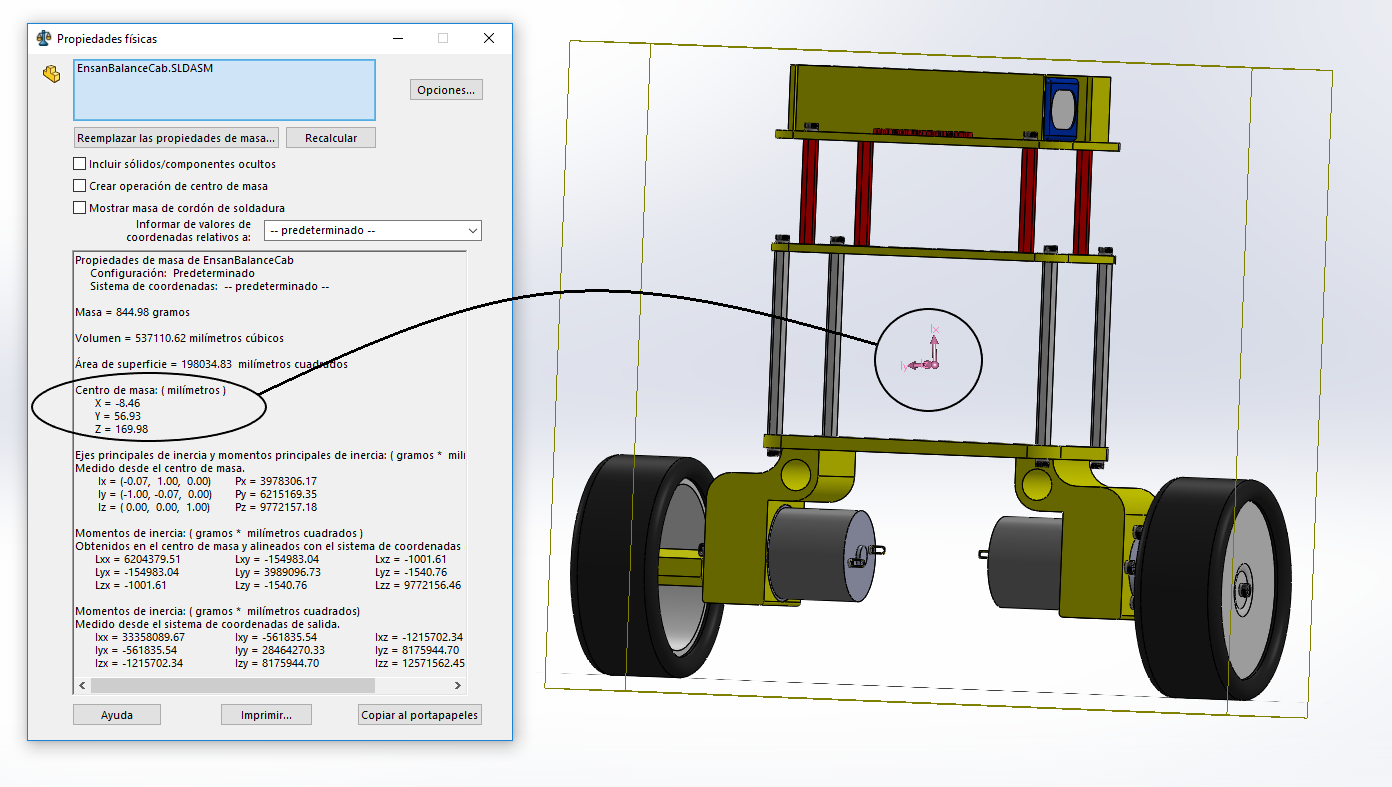
\includegraphics[scale=0.3]{imagenes/Balancing_robot/center_mass}
	\end{figure}
\end{frame}

\begin{frame}{Obtención ángulo}
\begin{block}{}
	\begin{itemize}
		\item Para corregir el ángulo es necesario el conocimiento de este en cada instante.\pause
		\item Unidad de medida incercial (IMU) \pause
	\end{itemize}
\end{block}
\begin{alertblock}{}
	\centering \textbf{MPU6050} \pause
\end{alertblock}
	\begin{center}
	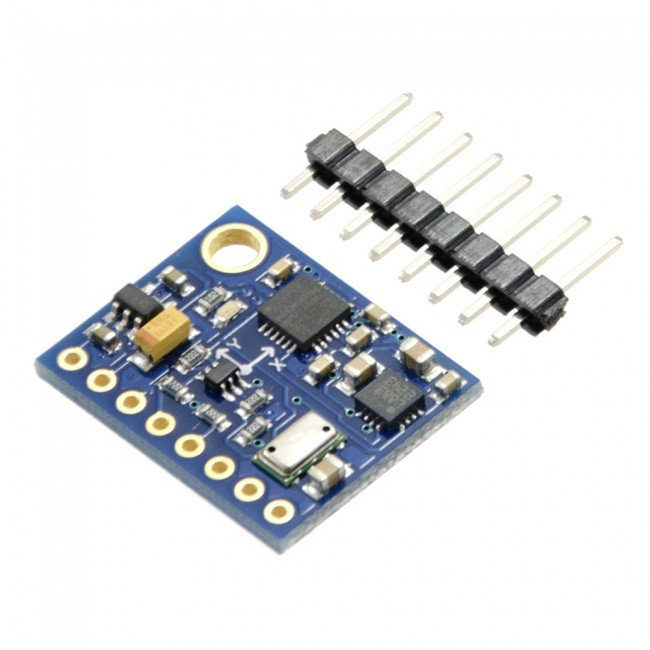
\includegraphics [width =0.3\textwidth ]{imagenes/EstadoArte/IMU1}
\end{center}
\end{frame}

\begin{frame}{Obtención ángulo}
		\begin{block}{}
			\begin{itemize}
				\item 6DOF \pause
				\item Acelerómetro y giroscopio \pause
				\item Comunicación I2C \pause
				\item Uso de DMP solo para Arduino \pause
			\end{itemize}
		\end{block}
		\begin{alertblock}{}
			\centering \textbf{MEJOR OPCIÓN CON ARDUINO} 
		\end{alertblock}
\end{frame}

\begin{frame}{Obtención ángulo}
	\begin{figure}[H]
		\center
		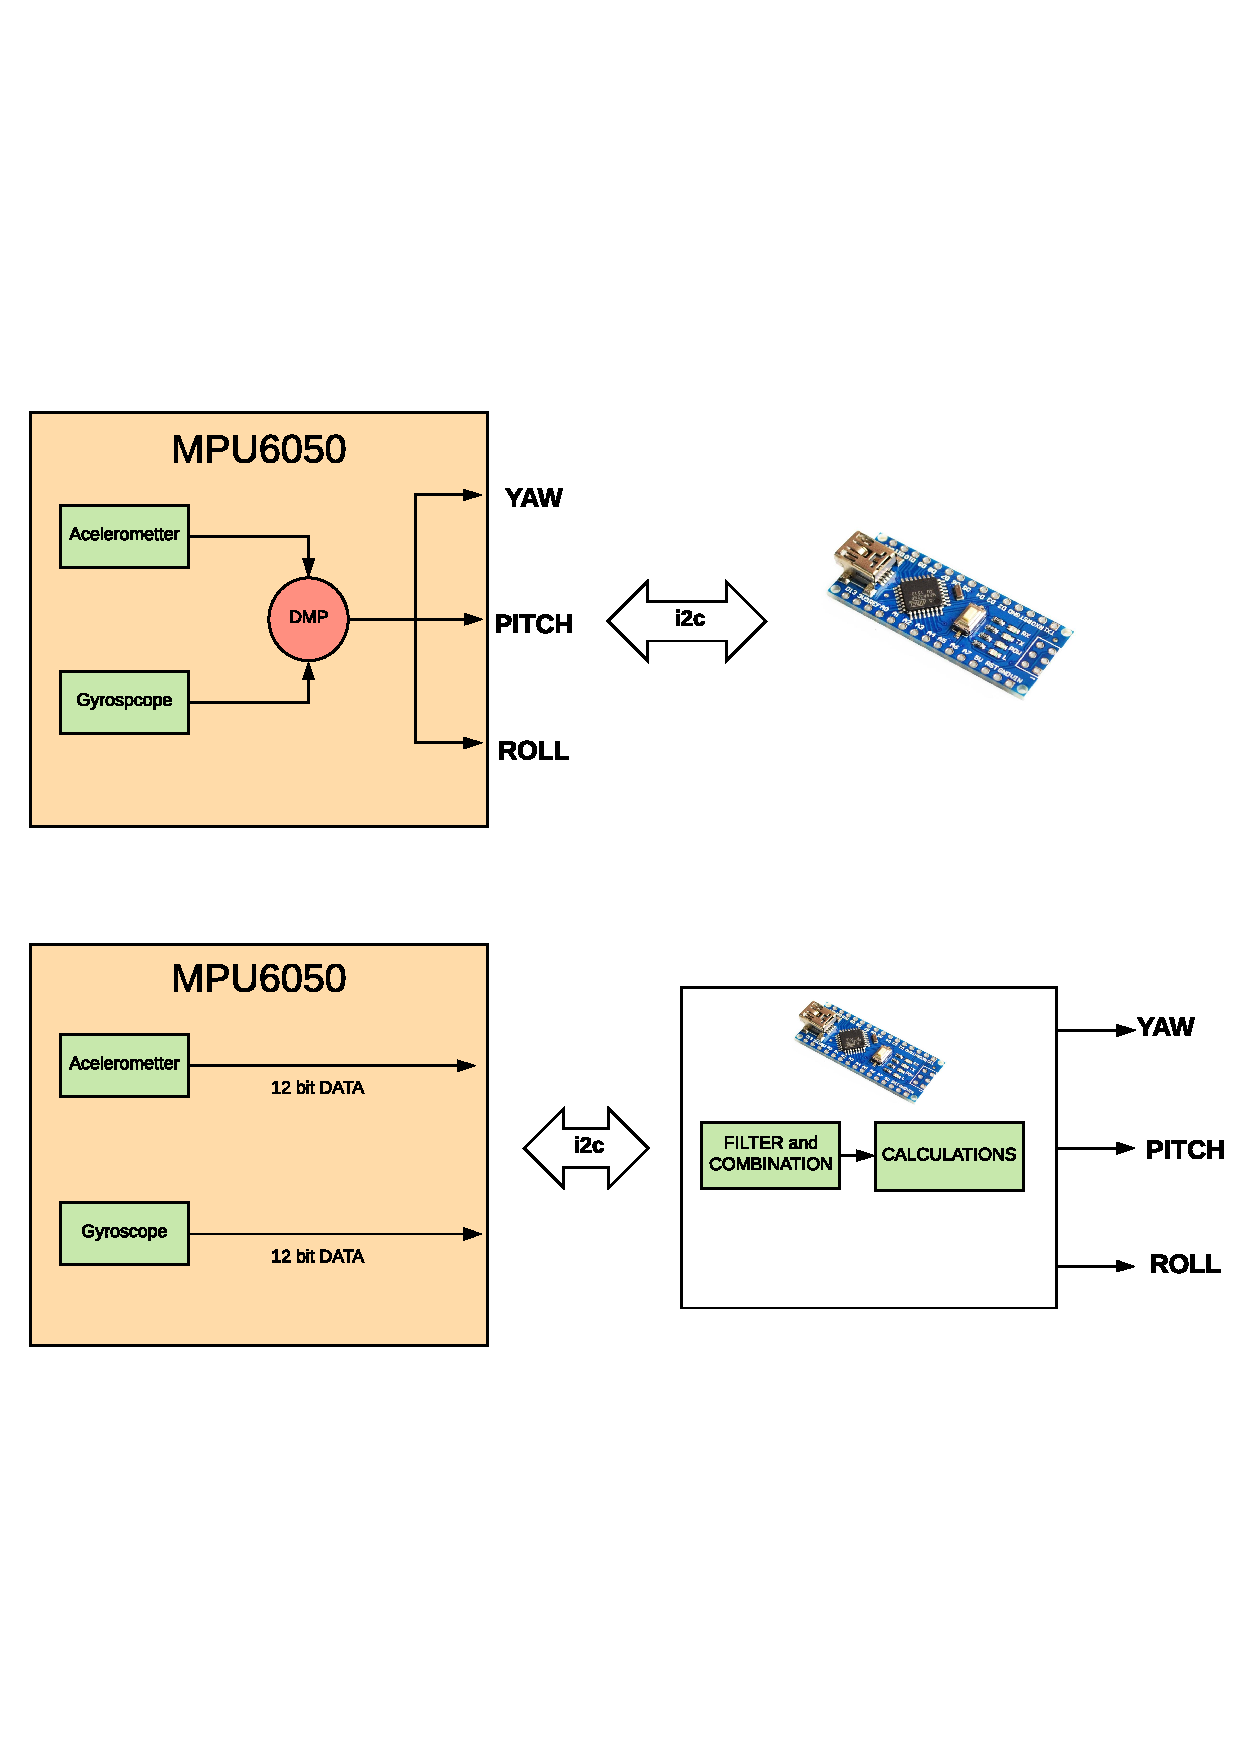
\includegraphics[trim = 0mm 5cm 0mm 5cm, clip,scale=0.4]{imagenes/Balancing_robot/DMPexample.pdf}
	\end{figure} 
\end{frame}


\begin{frame}{Coexistencia microcontrolador-FPGA}
\begin{block}{}
	\begin{itemize}
		\item Ángulo obtenido por Arduino-Nano \pause
		\item FPGA necesita conocer el ángulo \pause
	\end{itemize}
\end{block}
\begin{alertblock}{}
	\centering \textbf{Coexistencia microcontrador-FPGA}  \pause
\end{alertblock}
\begin{alertblock}{}
	\centering \textbf{Paralelizar los procesos que pueden ser paralelizados} \pause 
\end{alertblock}
\end{frame}


\begin{frame}{Coexistencia microcontrolador-FPGA}
	\begin{figure}[H]
		\center
		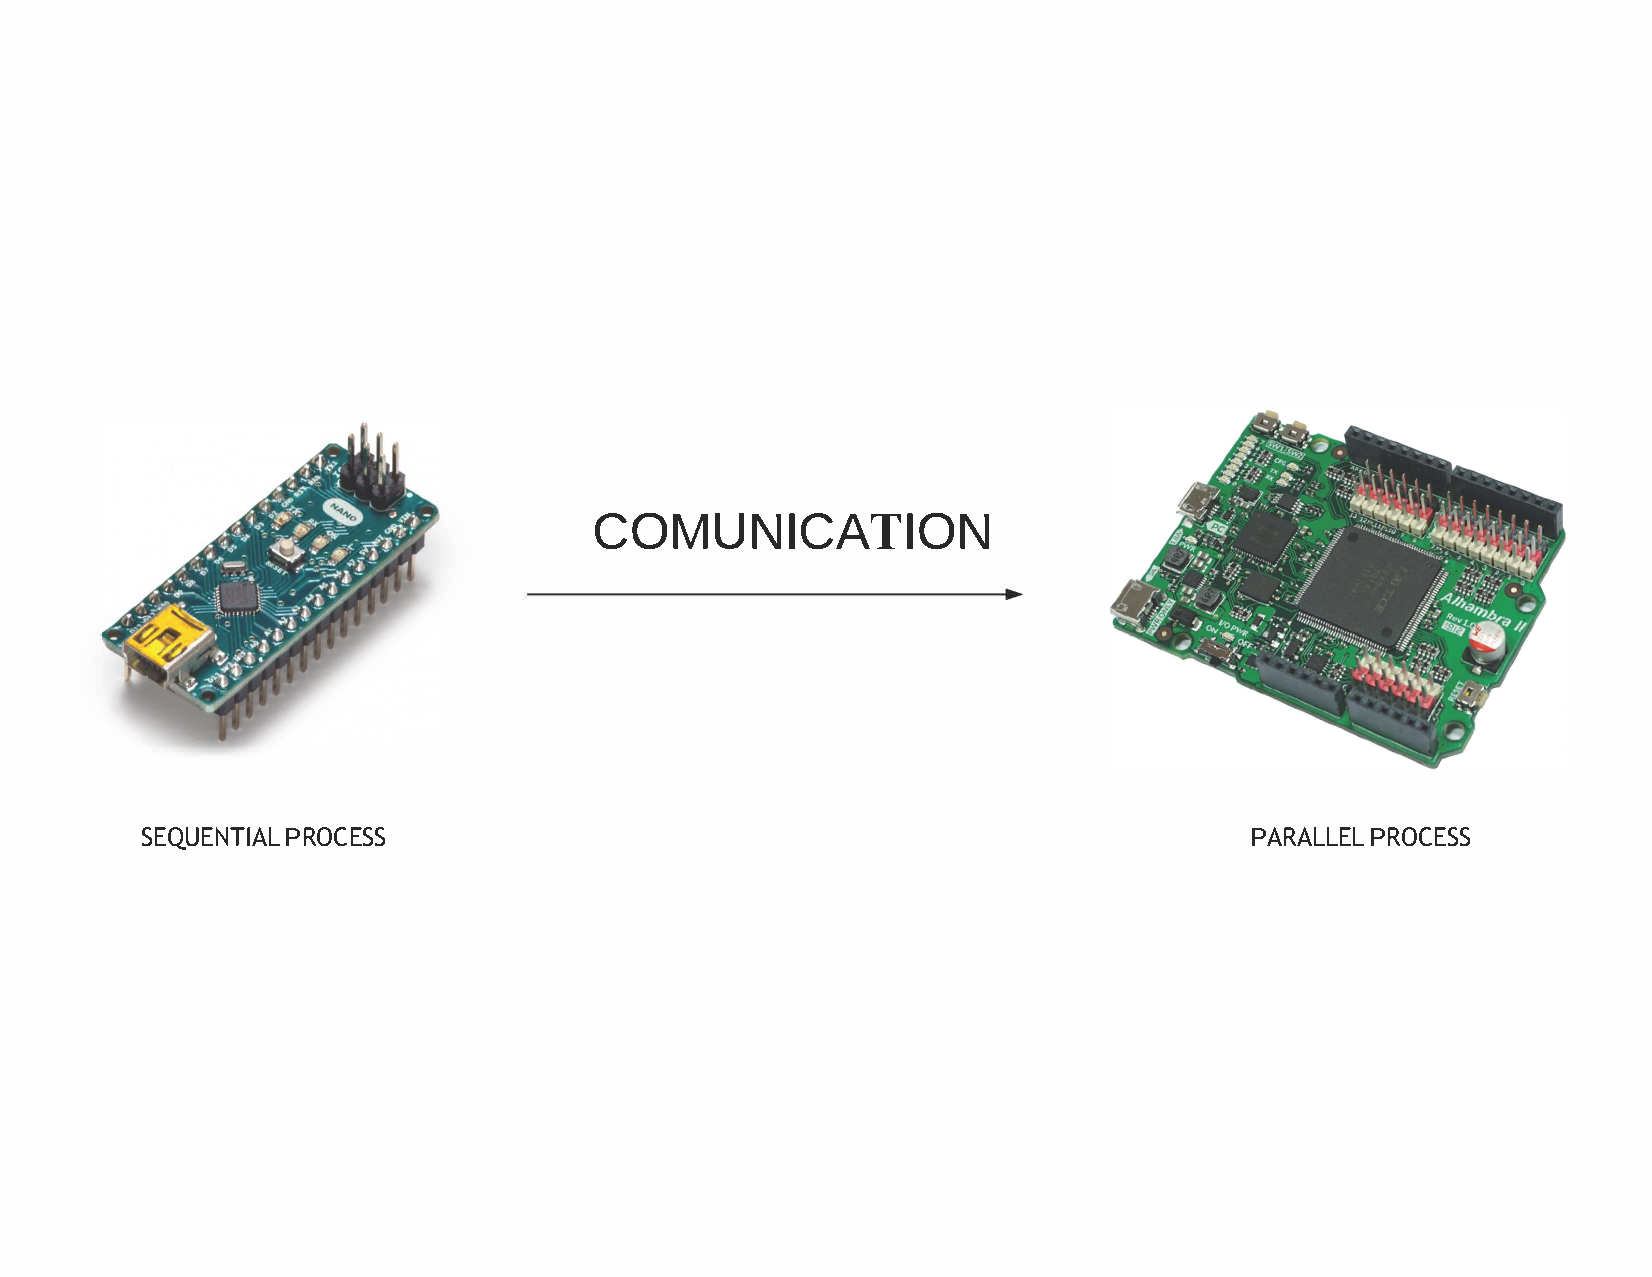
\includegraphics[trim = 0mm 40mm 0mm 20mm, clip,scale=0.4]{imagenes/Balancing_robot/coexistencia1.pdf}
	\end{figure}
\end{frame}

\begin{frame}{Coexistencia microcontrolador-FPGA}
\begin{figure}[H]
	\center
	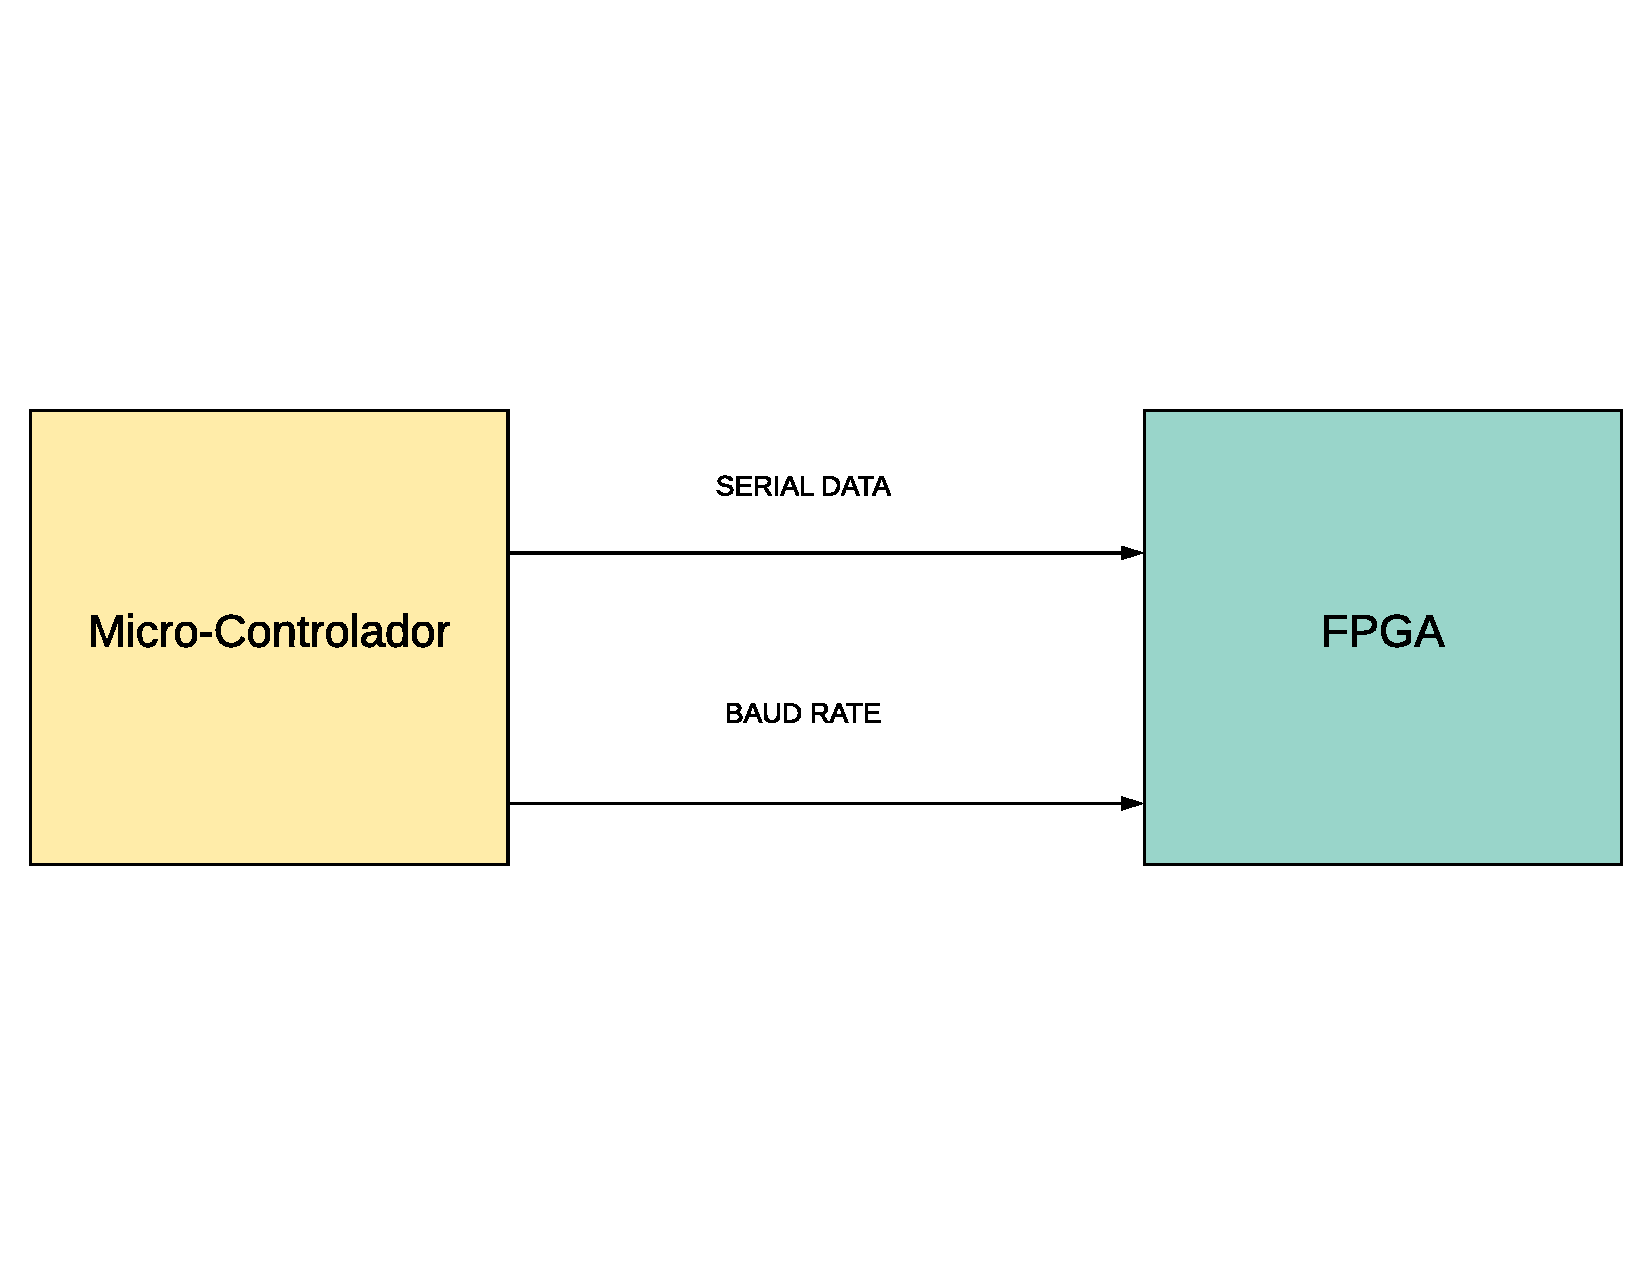
\includegraphics[trim = 0mm 40mm 0mm 20mm, clip,scale=0.3]{imagenes/Balancing_robot/coexistencia2.pdf}
\end{figure}
\begin{center}
	\begin{figure}[H]
		\center
		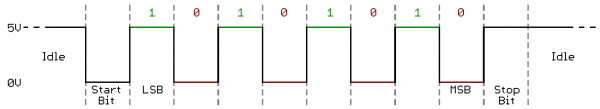
\includegraphics[scale=0.75, angle=0]{imagenes/Balancing_Robot/serial_comunicattion.png}
	\end{figure}
\end{center}
\end{frame}

\begin{frame}{Coexistencia microcontrolador-FPGA}
		\centering \textbf{Desde el punto de vista del microcontrolador}
		\begin{figure}[H]
			\center
			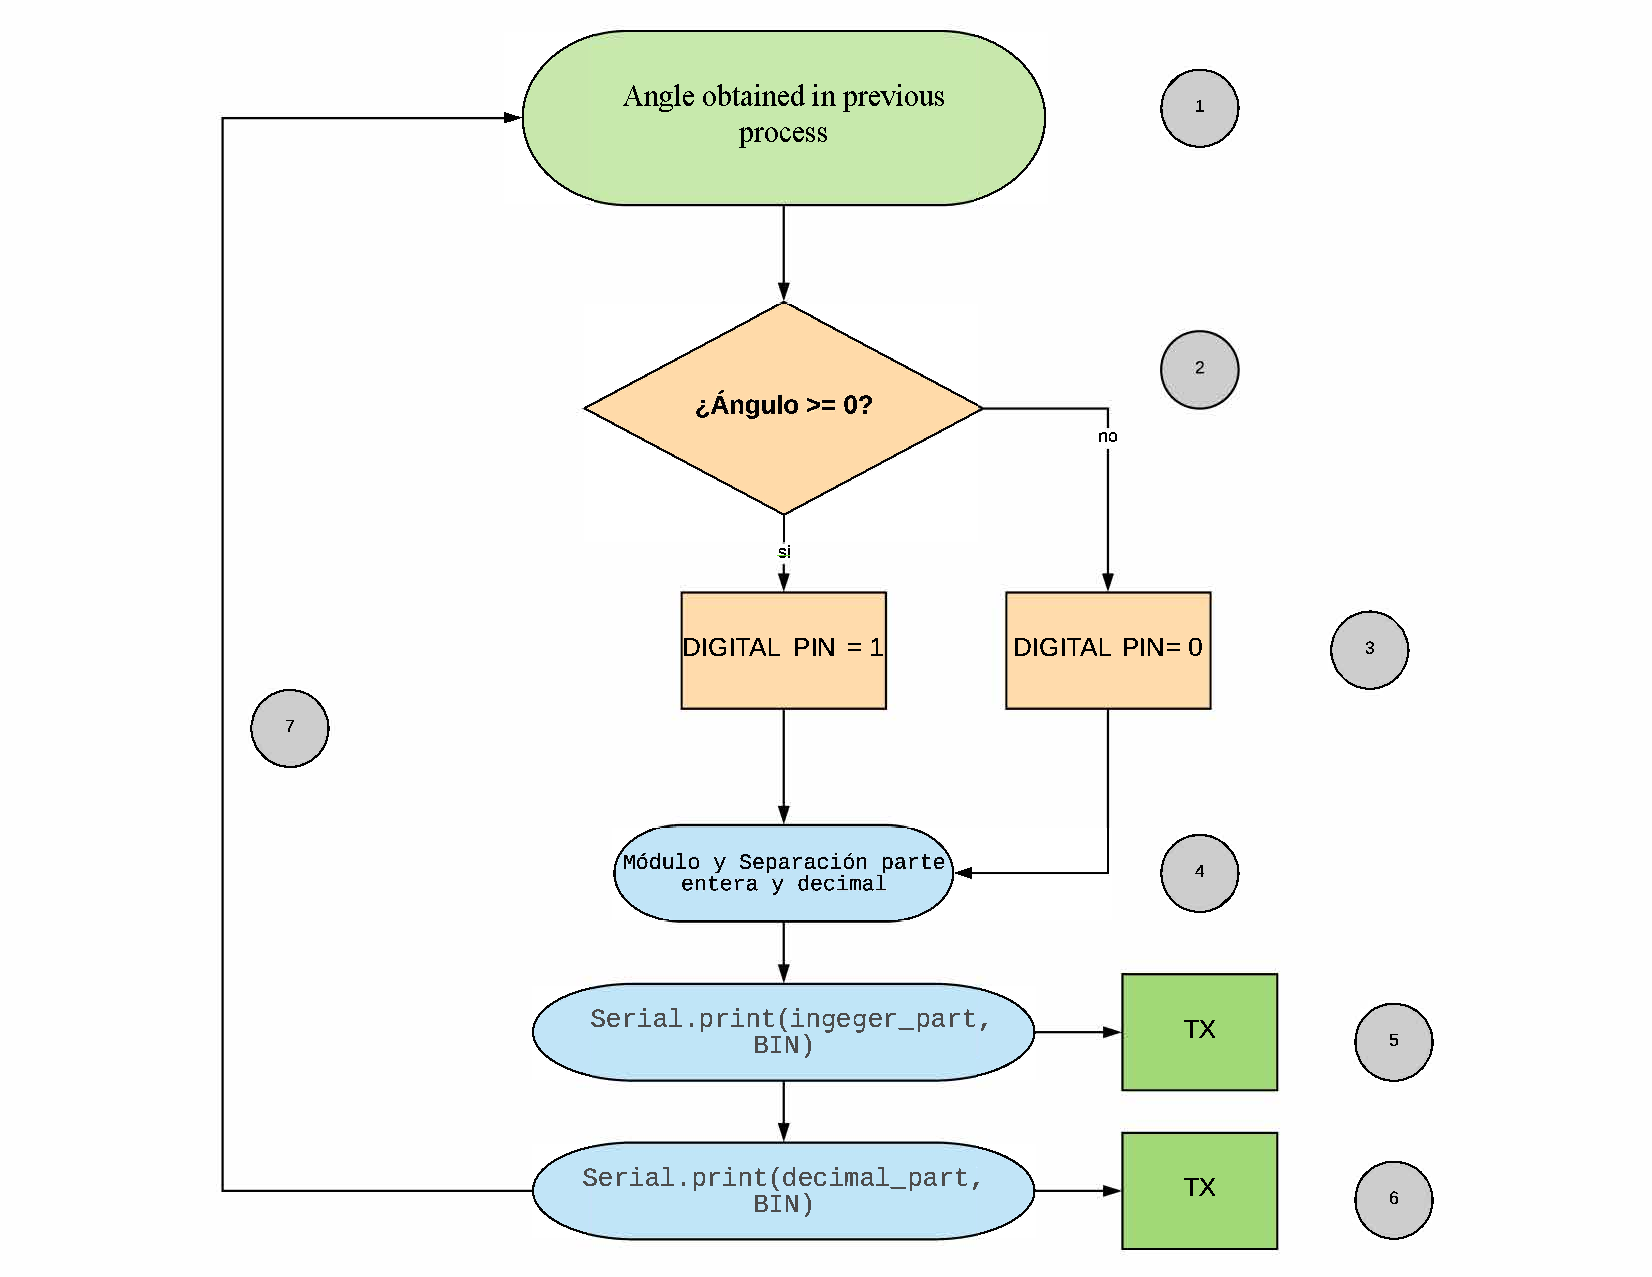
\includegraphics[trim = 0mm 0mm 0mm 0mm, clip,scale=0.3]{imagenes/Balancing_robot/extraccion_angulo.pdf}
		\end{figure}
\end{frame}

\begin{frame}{Coexistencia microcontrolador-FPGA}
\centering \textbf{Desde el punto de vista de la FPGA}
\begin{center}
	\begin{figure}[H]
		\center
		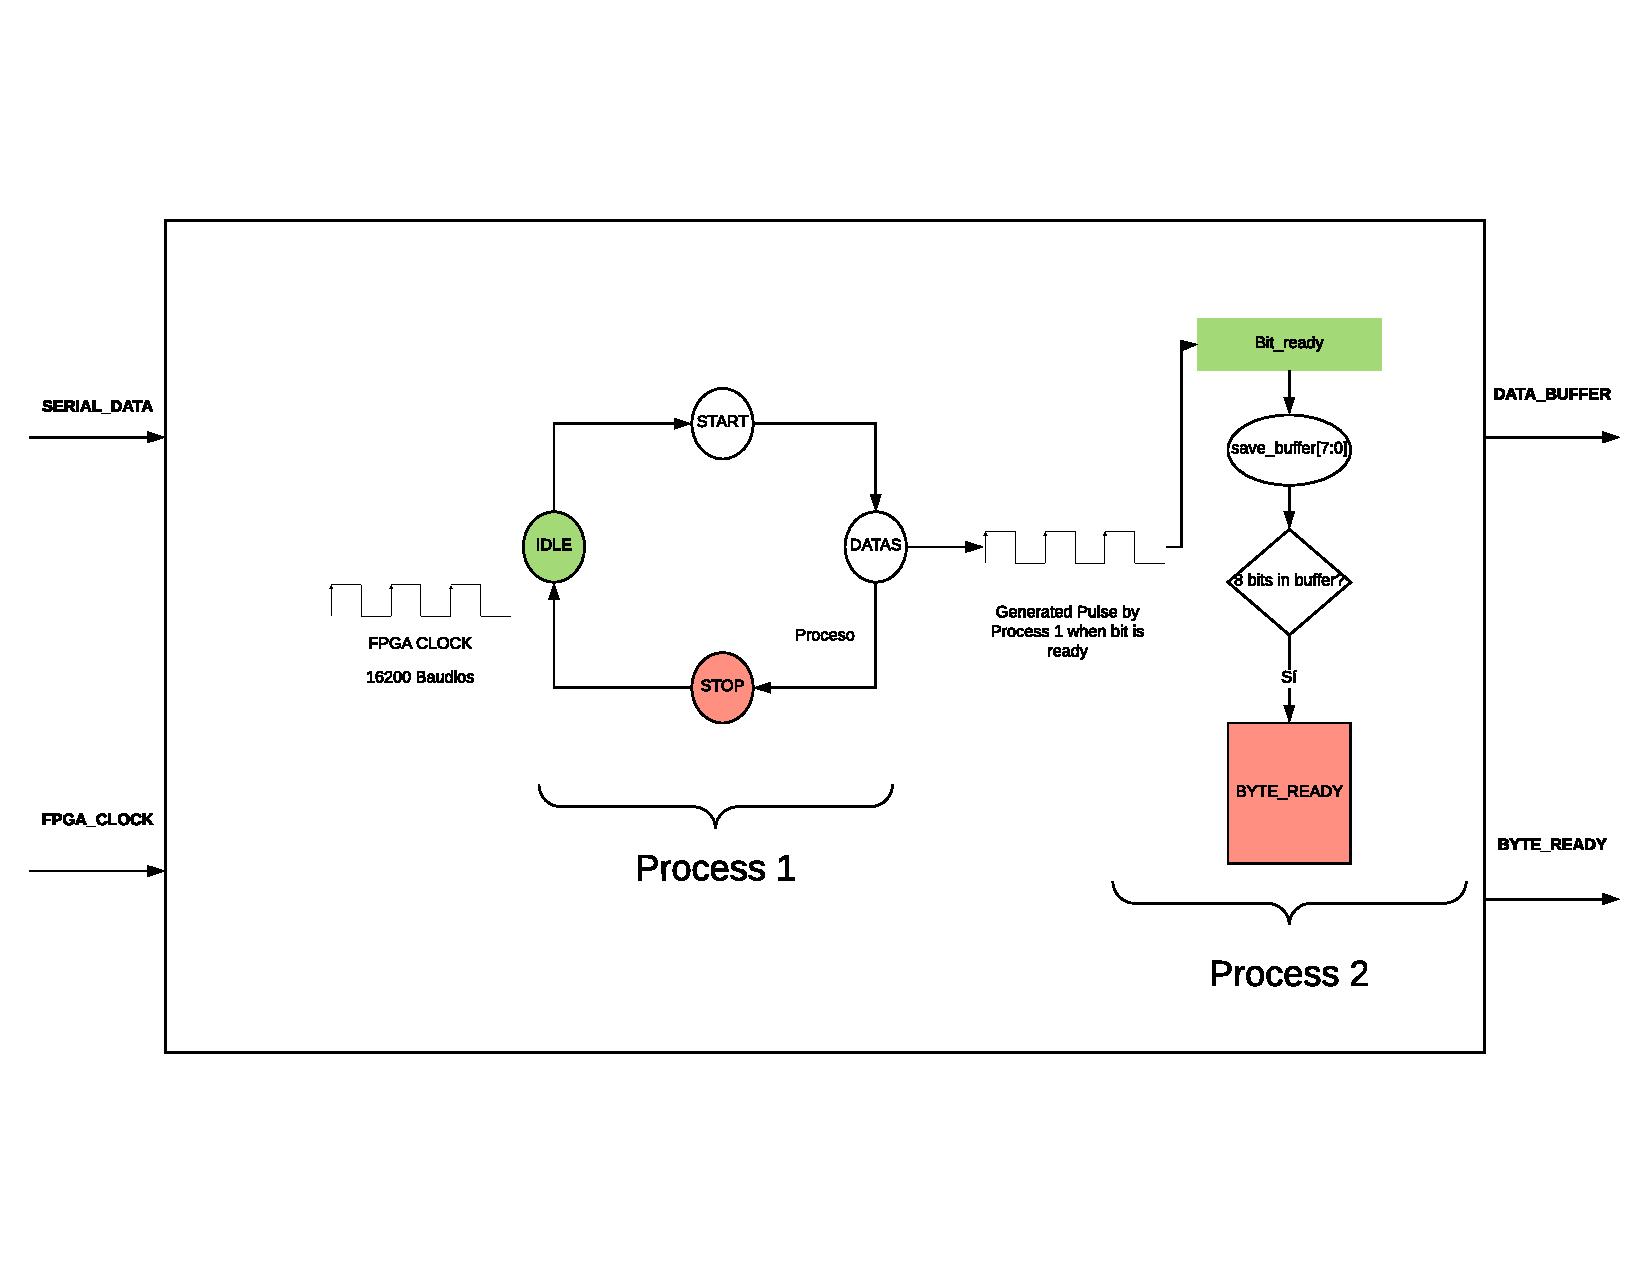
\includegraphics[trim = 0mm 0mm 0mm 10mm, clip,scale=0.4, angle=0]{imagenes/Balancing_robot/arduino_interfacefluid.pdf}

	\end{figure}
\end{center}
\end{frame}

\begin{frame}{Coexistencia microcontrolador-FPGA}
\centering \textbf{Aspecto en IceStudio de la comunicación}
\begin{figure}[H]
	\center
	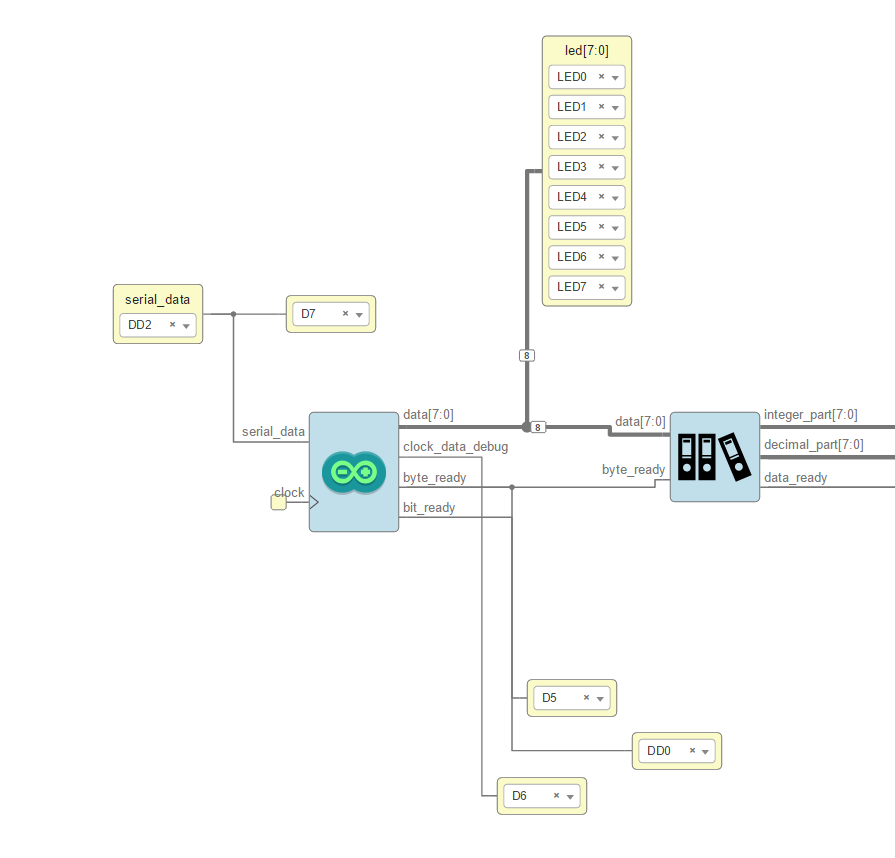
\includegraphics[scale=0.3]{imagenes/Balancing_robot/arduino_arrange.PNG}
\end{figure}
\end{frame}





\begin{frame}{Control PID}
\begin{block}{}
	\begin{itemize}
		\item Necesidad de minimizar el ángulo, en este caso a 0º
		\item Surgen muchas opciones, lógica fuzzy, algoritmos genéticos, PID
		\item PID por su fácil implementación y paralelismo
	\end{itemize}
\end{block}
\begin{alertblock}
	\centering \textbf{PID por su fácil implementación y paralelismo}
\end{alertblock}
\end{frame}

\begin{frame}{Control P}
		\begin{figure}[H]
		\center
		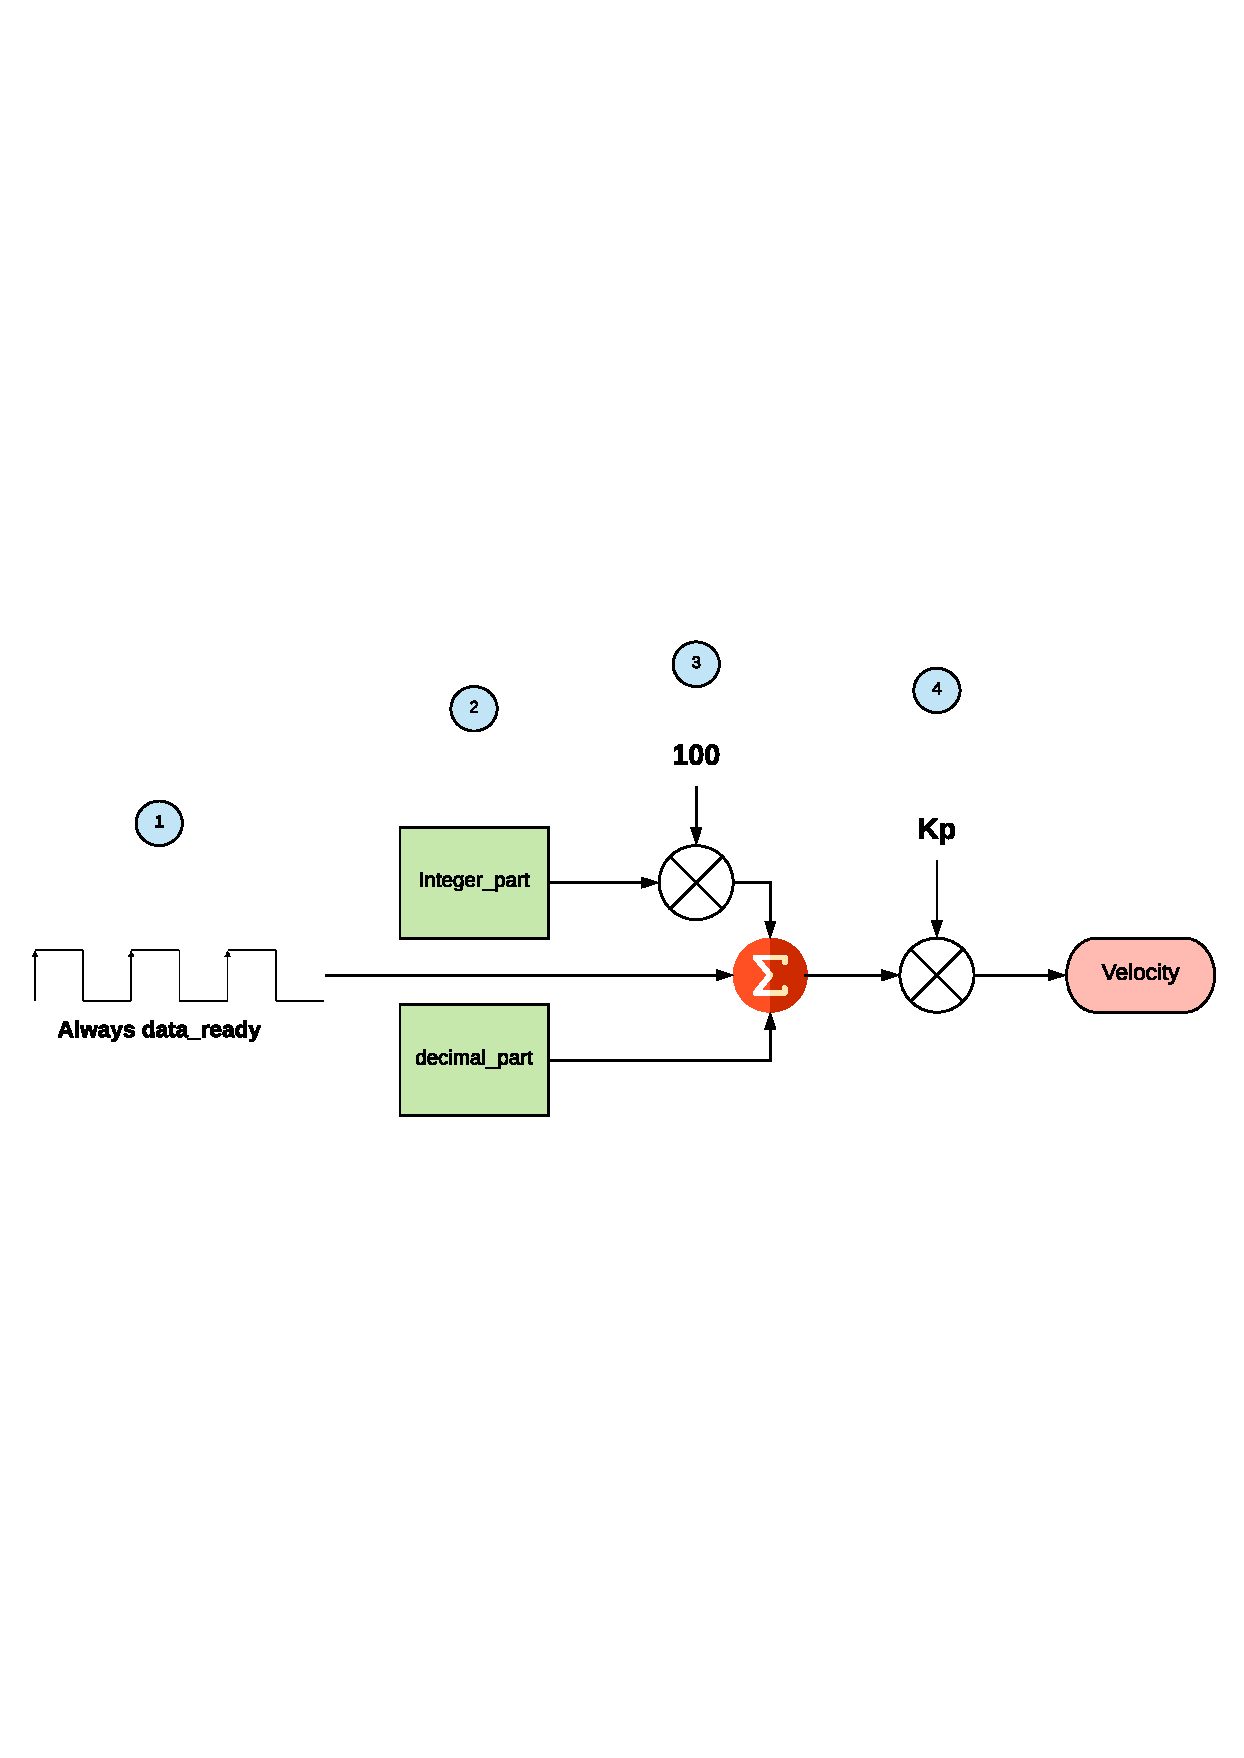
\includegraphics[trim = 0cm 7cm 0mm 7cm, clip,scale=0.5]{imagenes/Balancing_robot/P.pdf}
		\end{figure}
\end{frame}

\begin{frame}{Control D}
			\begin{figure}[H]
			\center
			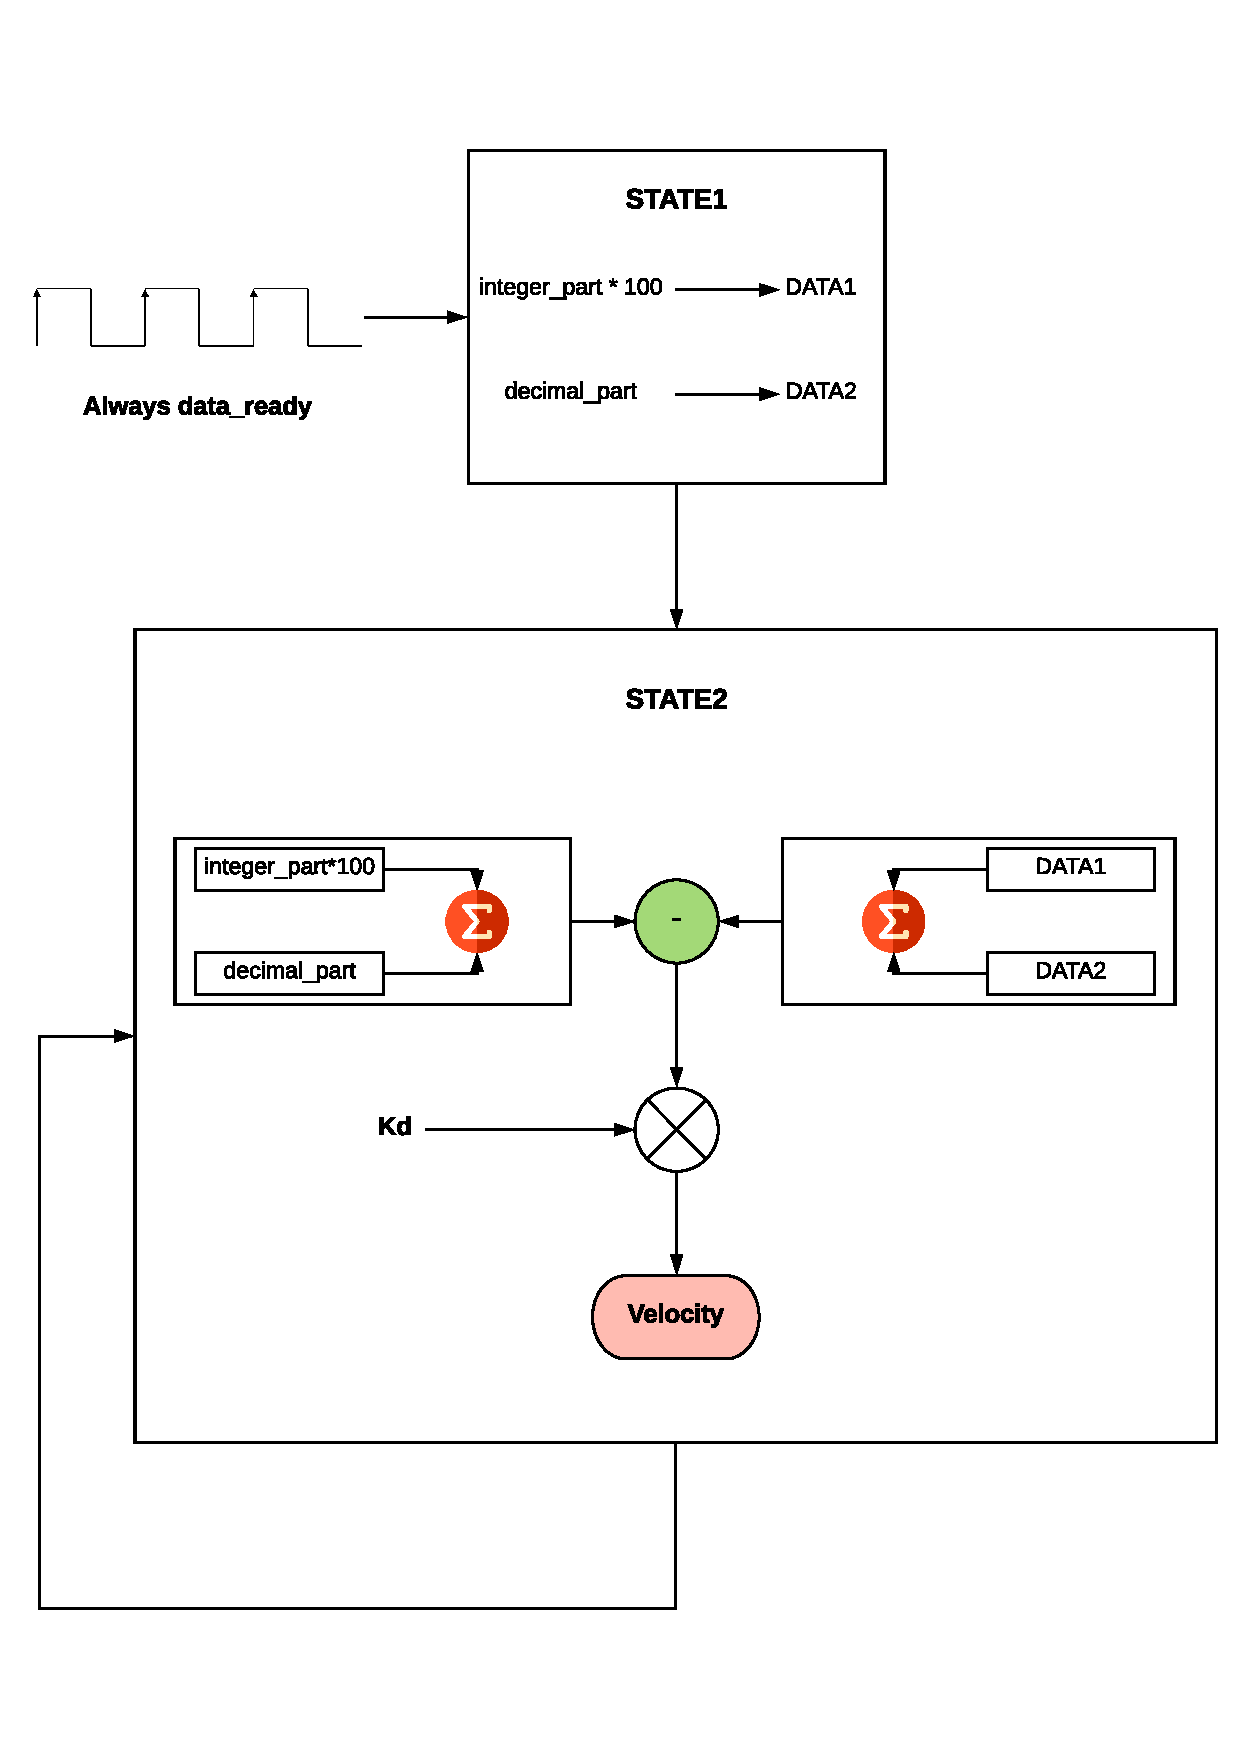
\includegraphics[trim = 0cm 0cm 0mm 2cm, clip,scale=0.3]{imagenes/Balancing_robot/D.pdf}
		\end{figure}
\end{frame}

\begin{frame}{Control PD}
	\begin{figure}[H]
		\center
		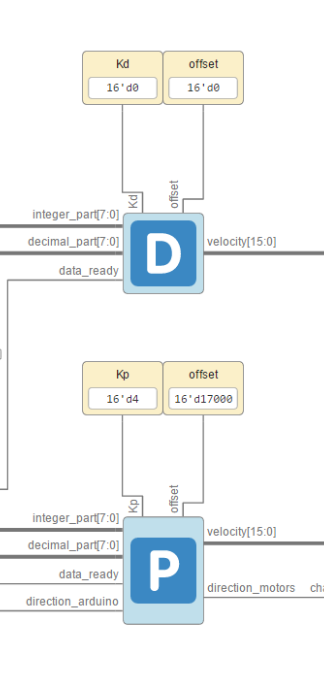
\includegraphics[trim = 0cm 0cm 0mm 0cm, clip,scale=0.5]{imagenes/Balancing_robot/PDControl.PNG}
	\end{figure}
\end{frame}



\begin{frame}{Control de los motores}
\begin{block}{}
	\begin{itemize}
		\item Traducción de la salida del PD, velocidad y sentido de motores DC \pause
	\end{itemize}
\end{block}
\centering \textbf{MC33926}
		\begin{figure}[H]
			\center
			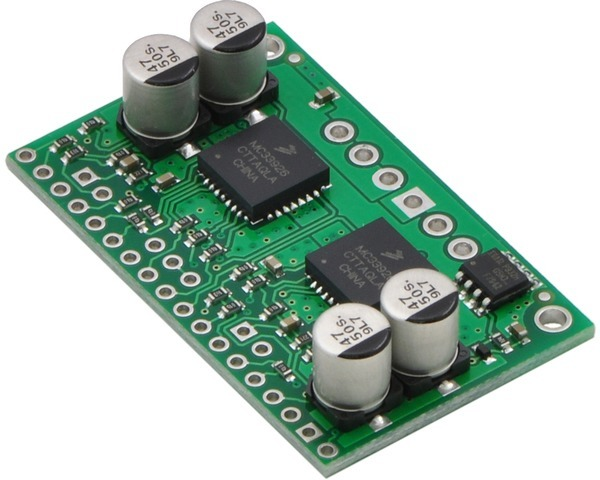
\includegraphics[trim = 0mm 0cm 0mm 0cm, clip,scale=0.2]{imagenes/Balancing_robot/driver_motor.jpg} \pause
		\end{figure}

\begin{alertblock}{}
	\begin{itemize}
		\item Como entradas: \begin{itemize}
			\item Señal PWM \pause
			\item Sentido de giro \pause
		\end{itemize}
		\item Como salidas: \begin{itemize}
		\item Movimiento de los motores 
	\end{itemize}
	\end{itemize}
\end{alertblock}
\end{frame}


\begin{frame}{Módulo PWM}
	\begin{figure}[H]
		\center
		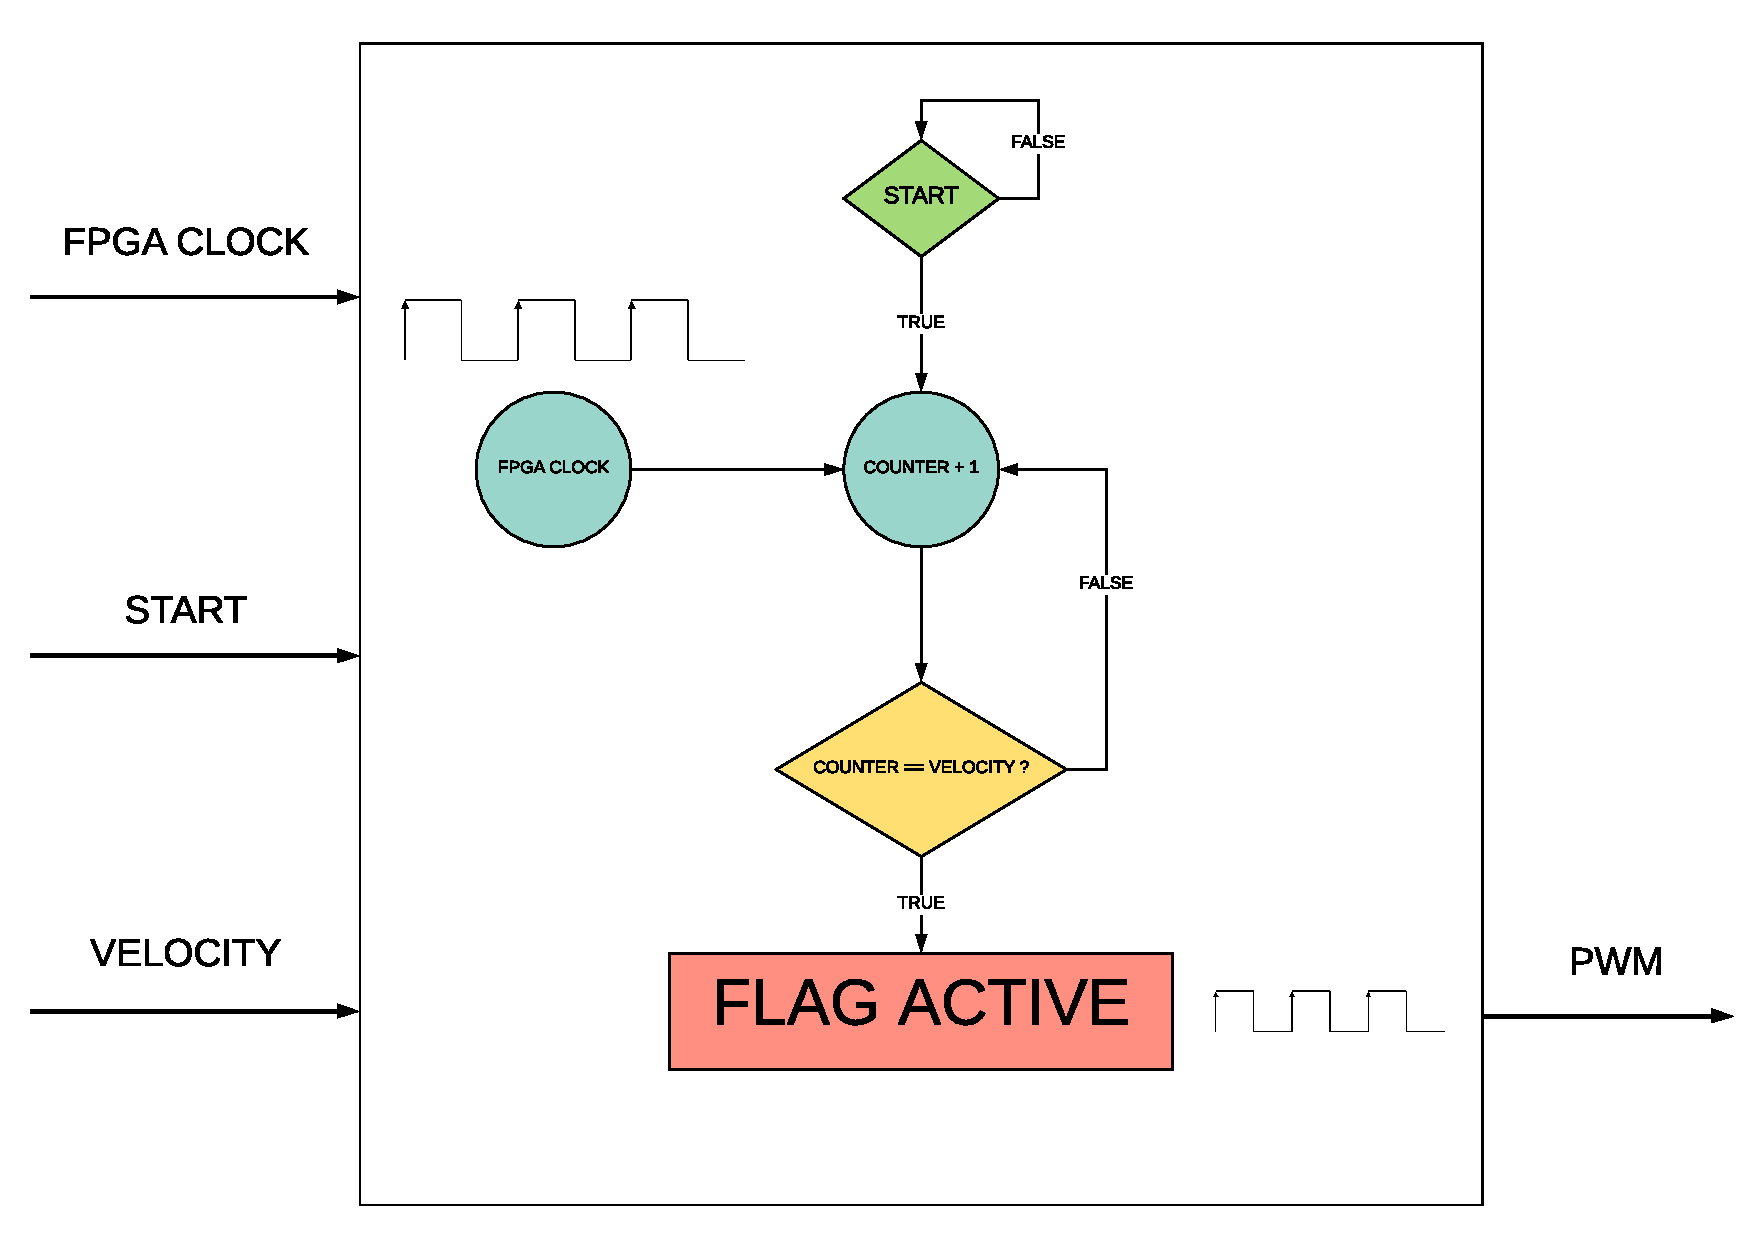
\includegraphics[trim = 0mm 0mm 0mm 0mm, clip,scale=0.4]{imagenes/Balancing_robot/pwm_control.pdf}
	\end{figure}
\end{frame}

\begin{frame}
	\begin{figure}[H]
		\center
		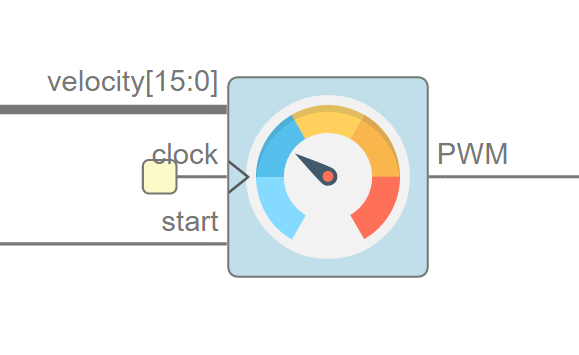
\includegraphics[scale=0.5]{imagenes/Balancing_robot/PWM_module.PNG}
	\end{figure}
\end{frame}


\begin{frame}{Diseño e implementación PCB}
Hay demasiados cables sueltos y hacemos una PCB, porque 4 capas, porque jumpers, porque posibilidad para 4 motores.
\end{frame}
\subsection{Experimentos y sistema final}
\begin{frame}{Impresión, montaje y ensamblado}
Fotos del ensamblado y vídeo final del sistema.
Debería meter aquí el módulo VGA que hice para aprender y el control de brushless?	
\end{frame}
%%%%%%%%%%%%%%%%%%%%%%%%%%%%%%%%%%%%%%%%%%%%%%%%%%%%%%%%%%%%%%%%%%%%
\section{Cuadricóptero con visión artificial}
\begin{frame}{Diseño del sistema}
Dejar claro que como ha sobrado tiempo, se hace esto para que no piensen que no hemos llegado. Diagrama de bloques general y separación entre percepción y control.
\end{frame}
\subsection{Implementación de la percepción}
\begin{frame}{OV7670 y protocolo I2C}
Porque se ha usado esa cámara, y se dice que se ha implementado un protocolo i2c necesario para los registros, me tire dos meses con ello y tiene que salir :). Se muestra diagrama de bloques del i2c
\end{frame}
\begin{frame}{Reconocimiento del volumen y posición}
Las formulas básicas de como hemos hecho esa percepción y la ventaja de hacer eso con una FPGA, no se necesita memoria externa. 
\end{frame}
\subsection{Diseño del control}
\begin{frame}
Se deja claro que esto falta por implementar pero todo el diseño esta propuesto y debería funcionar. Se explica rápido.
\end{frame}
\section{Conclusiones y trabajo futuro}
\begin{frame}{Conclusiones}
Conclusiones de este trabajo
\end{frame}
\begin{frame}{Trabajo futuro}
Posible trabajo futuro
\end{frame}
\end{document}


